\documentclass[a4paper, 12pt]{article}

%%%%%%%%%%%%%%%%%%%%%%%%%%%%%%% PACKAGES %%%%%%%%%%%%%%%%%%%%%%%%%%%%%%%
% Math-related things
\usepackage{amsmath}
\usepackage{amssymb}
\usepackage{amsthm}
% Italian spelling
\usepackage[italian]{babel}
% Accenti e caratteri speciali
\usepackage[utf8x]{inputenc}
% Margini e grafica della pagina
\usepackage[top=2cm, bottom=2cm, left=2cm, right=2cm]{geometry}
\usepackage{fancyhdr}
% Tabelle
\usepackage{tabularx}
\usepackage[table]{xcolor}
% Graphs and Images handling
\usepackage{graphicx}
\usepackage{svg}
% VHDL language support
\usepackage{minted}
% Hypertext references
\usepackage{hyperref}
% Citations
\usepackage{epigraph}

% Contents page settings
\renewcommand*\contentsname{Indice}
\setcounter{tocdepth}{3}

\newcommand{\quantities}[1]{%
	\begin{tabular}{@{}c@{}}\strut#1\strut\end{tabular}%
}

% General page settings
\pagestyle{fancy}
\fancyhf{}
\rhead{\leftmark}
\lhead{Eriantys - Prova Finale di Ingegneria del Software}
\cfoot{\thepage}

% Hyperrefs setup
\hypersetup{
	colorlinks=true,
	linkcolor=[HTML]{7390A6}, %254 101 23 | #7390A6
	filecolor=magenta,      
	urlcolor=[HTML]{4e42f5},
	citecolor=[HTML]{384f9c},
	pdftitle={Eriantys - Prova Finale di Ingegneria del Software},
	pdfpagemode=FullScreen,
}

% Tables settings
\setlength{\arrayrulewidth}{1mm}
\setlength{\tabcolsep}{5pt}
\renewcommand{\arraystretch}{2.5}
\arrayrulecolor[HTML]{211d1b}

\begin{document}
	\pagenumbering{gobble}
	\thispagestyle{empty} % serve per rimuovere tutte le impostazioni delle pagine dalla prima pagina
	
	% FRONTESPIZIO
	\begin{center}
		% Intestazione
		\Large{\textbf{Politecnico di Milano}} \\
		\vspace{-4mm}
		\rule{\textwidth}{0.4pt}
		\normalsize{SCUOLA DI INGEGNERIA INDUSTRIALE E DELL’INFORMAZIONE} \\
		\normalsize{Laurea Triennale -- Ingegneria Informatica} \\
		\vspace{20mm}
		% Logo Politecnico
		\begin{figure}[h!]
			\centering
			
\includegraphics[height=0.30\textheight]{logo_poli_bianco}
		\end{figure}
		\vspace{12mm}
		% Titolo Tesi
		\huge{\textbf{Eriantys}} \\
		\vspace{22mm}
	\end{center}
	
	% Docente
	\begin{flushleft}
		\normalsize{Supervisore} \\
		\small{\textbf{Professor Gianpaolo Cugola}} \\
	\end{flushleft}
	\vspace{10mm}
	
	% Autore
	\begin{flushright}
		\normalsize{Candidati} \\
		\small{\textbf{Alberto PADDEU -- 10729194}} \\
		\small{\textbf{Paolo PERTINO -- 10729600}} \\
		\small{\textbf{Leonardo PESCE -- 10659489}} \\
	\end{flushright}
	\vspace{15mm}
	
	% Piè Di Pagina
	\begin{center}
		\rule{\textwidth}{0.4pt}
		\small{\textbf{Anno Accademico 2021 -- 2022}}
	\end{center}

	\newpage
	\thispagestyle{plain}
	{\transparent{0.4}\vspace*{11.0cm}\hspace*{-6cm}
\includegraphics[width=0.85\paperwidth]{./raggiera_polimi.pdf}}
	
	\newpage
	\pagenumbering{arabic}
	
	\tableofcontents
	
	\newpage
	\section{Introduzione}
	\subsection{Obiettivi}
	\paragraph{}
	La \textbf{Prova Finale di Ingegneria del Software} dell'anno scolastico 2021-2022 prevede lo sviluppo di una versione software del gioco da tavolo \emph{Eriantys}, un prodotto \emph{Cranio Creations}\cite{eriantys} che si ispira e tenta di rinnovare il già affermato \emph{Carolus Magnus}\cite{carolusMagnus}.
	
	\paragraph{}
	Il prodotto finale dovrà soddisfare i requisiti \emph{Game-Specific} e \emph{Game-Agnostic} indicati nel documento \emph{requirements.pdf}. In particolare è richiesto l'utilizzo del design pattern \emph{Model-View-Controller} di cui a breve forniremo una concisa descrizione.\\
	Per incrementare il punteggio ottenuto, il team si concentrerà nell'implementazione delle regole complete del gioco, nel fornire la possibilità ai giocatori di connettersi al server e giocare tramite un'interfaccia a linea di comando (CLI) oppure mediante l'interazione con un'interfaccia grafica (GUI). Infine si darà spazio all'implementazione di quante più possibili delle seguente funzionalità aggiuntive: \emph{12 carte personaggio, partite a 4 giocatori, partite multiple e persistenza}.
	
	\subsection{Model-View-Controller}
	\paragraph{}
	Il \emph{Model-View-Controller} è un design pattern per la progettazione di un'architettura software. Esso permette di separare la logica di presentazione dell'applicativo da quella applicativa(o detta di business).\\
	\begin{figure}[h!]
		\centering
		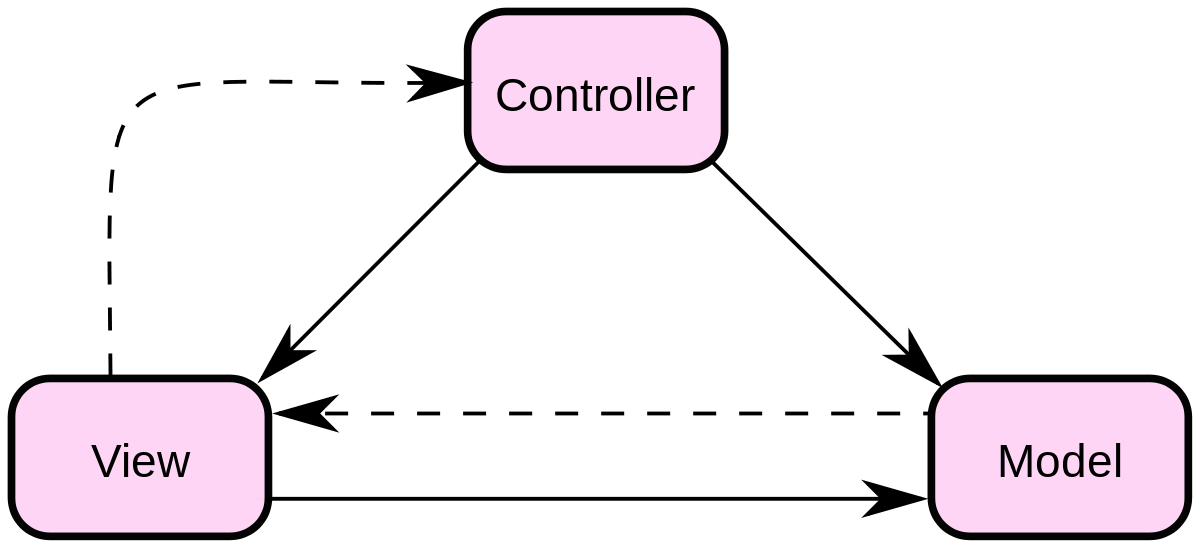
\includegraphics[scale=0.25]{mvc.png}
		\caption{Model-View-Controller Pattern}
	\end{figure}
	
	Come deducibile dal nome, tale architettura è strutturata su 3 differenti layer:\\
	\begin{enumerate}
		\item \emph{Model} - gestione diretta dei dati, della logica e delle regole del programma. Si noti come l'utente non modifica in modo diretto lo stato del model, bensì si interfaccia con il controller il quale gestisce in separata sede l'interazione con lo stato interno del sistema;
		\item \emph{View} - permette la visualizzazione dello stato del model e gestisce l'interazione con gli utenti e agenti esterni; 
		\item \emph{Controller} - riceve i comandi dell'utente attraverso la view e li attua modificando gli stati degli altri due layers.
	\end{enumerate}
	Sono possibili viste multiple di uno stesso modello. Nel nostro caso, infatti, saranno implementate due viste: il gioco sarà pertanto accessibile sia attraverso linea di comando sia mediante interfaccia grafica.
	
	\subsection{Installazione}
	\subsubsection{Requisiti di sistema}
	\paragraph{}
	Per poter installare l'applicazione è necessario aver già predisposti sul proprio computer:
	\begin{itemize}
		\item \textbf{Sistema Operativo}: Windows 10/11 oppure Linux (testato su Ubuntu 18.04);
		\item \textbf{Java}: Java SE JDK 17;
		\item \textbf{Maven}: Maven 3.x;
		\item \textbf{Risoluzione schermo}: 1920x1080 (fortemente raccomandata).
	\end{itemize}
	\subsubsection{Installazione su Windows}
	\paragraph{}
	L'installazione dell'applicativo su Windows prevede due passaggi:
	\begin{enumerate}
		\item \textbf{Abilitare i codici ANSI sulla console}:
			  \begin{itemize}
			  	  \item Premere i tasti Windows ⊞ + R e digitare \textit{intl.cpl};
			  	  \item Nella finestra che si apre, cliccare \textit{Opzioni di Amministrazione} nella barra in alto;
			  	  \item Successivamente su \textit{Cambia le impostazioni locali di sistema...};
			  	  \item Spunta dunque la casella \textit{Beta: utilizzare Unicode UTF-8 per il supporto della lingua a livello mondiale};
			  	  \item Infine cliccare su \textit{Ok} e su \textit{Applica} per salvare i cambiamenti.
			  \end{itemize}
		
		\item \textbf{Installare il gioco generando i \textit{File Jar} relativi al Server e al Client}:
			  \begin{itemize}
			  	  \item Clonare la repo o scaricare il file zip;
			  	  \item Estrarre i file dall'archivio (solo se è stato scaricato il pacchetto zip dal punto precedente, altrimenti procedere con il prossimo step);
			  	  \item Aprire il terminale e navigare nella cartella estratta/della repo clonata utilizzando il comando:
				  \begin{minted}{bash}
	$ cd PATH/TO/ing-sw-2022-Pesce-Pertino-Paddeu
				  \end{minted}
			  	  \item Compila i file di gioco:
			  	  \begin{minted}{bash}
	$ mvn clean package
			  	  \end{minted}
			  \end{itemize}
	\end{enumerate}

	\subsubsection{Installazione su Linux}
	L'installazione del gioco in ambiente linux prevede i seguenti passaggi:
	\begin{itemize}
		\item Clonare la repo o scaricare il file compresso;
		\item Estrarre i file dall'archivio (solo se è stato scaricato il pacchetto compresso dal punto precedente, altrimenti procedere con il prossimo step);
		\item Aprire il terminale e navigare nella cartella estratta/della repo clonata utilizzando il comando:
		\begin{minted}{bash}
	$ cd PATH/TO/ing-sw-2022-Pesce-Pertino-Paddeu
		\end{minted}
		\item Compila i file di gioco:
		\begin{minted}{bash}
	$ mvn clean package
		\end{minted}
	\end{itemize}
	
	\newpage
	\subsection{Avvio dell'applicazione}
	\subsubsection{Requisiti per l'avvio dell'applicazione}
	\begin{itemize}
		\item \textbf{Java}: Java SE JDK 17;
		\item \textbf{Installazione}: aver seguito la procedura di installazione oppure aver scaricato i \textit{File Jar} precompilati presenti nella cartella \textit{Deliverables} presente sulla repository Github.
	\end{itemize}
	\subsubsection{Avvio del Server}
	\paragraph{}
	Una volta ottenuto il file \textit{softeng-GC3-ServerApp.jar}, aprire il terminale e spostarsi nella cartella in cui tale file è locato.
	Successivamente digitare:
	\begin{minted}{bash}
		$ java -jar softeng-GC3-ServerApp.jar <PORT_NUMBER>
	\end{minted}
	dove $<$\textit{PORT\_NUMBER}$>$ va sostituito con il numero di porta su cui si vuole aprire effettivamente il server (scegliere un numero intero compreso nell'intervallo [1024, 65535]).
	\paragraph{IMPORTANTE}: per far si che altre persone possano connettersi al server, potrebbe essere necessario fare \textit{port forwarding} della porta utilizzata al momento dell'avvio del server.
	
	\subsubsection{Avvio del Client}
	\paragraph{}
	Una volta ottenuto il file \textit{softeng-GC3-ClientApp.jar}, aprire il terminale e spostarsi nella cartella in cui tale file è locato.
	\paragraph{CLI}: per utilizzare la \textit{CLI} digitare:
	\begin{minted}{bash}
		$ java -jar softeng-GC3-ClientApp.jar cli
	\end{minted}
	\paragraph{GUI}: per usare la \textit{GUI} digitare:
	\begin{minted}{bash}
		$ java -jar softeng-GC3-ClientApp.jar gui
	\end{minted}
	
	\newpage
	\section{Consegna}
	\subsection{Funzionalità implementate}
	\paragraph{}
	Nella seguente sezione riportiamo una tabella contenente le funzionalità che abbiamo implementato corredate da una breve descrizione facendo riferimento a quella fornita nel documento dei requisiti.
	
	\begin{center}
		\begin{tabular}{ |p{4cm}|p{10cm}|p{2cm}| }
			\hline
			\rowcolor[HTML]{edeef0} \multicolumn{3}{|c|}{\textbf{Funzionalità Implementate}} \\
			\hline
			\rowcolor[HTML]{edeef0}
			\textit{Nome}& \textit{Descrizione} & \textit{Status} \\
			\hline
			\rowcolor[HTML]{edeef0}
			Regole complete & Il gioco deve essere giocabile da 2 o 3 giocatori, volendo con regole per esperti (devono venire implementate almeno 8 carte personaggio). & \cellcolor[HTML]{ACEDAA} \\
			\rowcolor[HTML]{edeef0}
			CLI & Il gioco deve essere giocabile da CLI. & \cellcolor[HTML]{ACEDAA} \\
			\rowcolor[HTML]{edeef0}
			GUI   & Il gioco deve essere giocabile da GUI. & \cellcolor[HTML]{ACEDAA} \\
			\rowcolor[HTML]{edeef0}
			Socket  & La connessione tra client e server deve avvenire attraverso socket TCP-IP. & \cellcolor[HTML]{ACEDAA} \\
			\rowcolor[HTML]{edeef0}
			\textbf{Carte Personaggio} & Implementare tutte e 12 le carte personaggio. & \cellcolor[HTML]{ACEDAA} \\
			\rowcolor[HTML]{edeef0}
			\textbf{4 Giocatori} & Realizzare il progetto in modo che sia possibile giocare partite da 2, 3 oppure 4 giocatori. & \cellcolor[HTML]{ACEDAA}    \\
			\rowcolor[HTML]{edeef0}
			\textbf{Partite multiple} & Realizzare il server in modo che possa gestire più partite \textbf{contemporaneamente}. & \cellcolor[HTML]{ACEDAA} \\
			\rowcolor[HTML]{edeef0}
			\textbf{Persistenza} & Lo stato di una partita deve essere salvato su disco, in modo che la partita possa riprendere anche a seguito dell'interruzione dell'esecuzione del server. & \cellcolor[HTML]{edaaaa} \\
			\rowcolor[HTML]{edeef0}
			\textbf{Resilienza alle disconnessioni} & I giocatori disconnessi possono ricollegarsi in seguito e continuare la partita. & \cellcolor[HTML]{edaaaa} \\
			\hline
		\end{tabular}
	\end{center}
	\paragraph{Legenda}: \fcolorbox{black}{green}{\rule{0pt}{6pt}\rule{6pt}{0pt}}\quad \textit{Implementato},  \fcolorbox{black}{red}{\rule{0pt}{6pt}\rule{6pt}{0pt}}\quad \textit{Non Implementato}
	\paragraph{}
	Sono state implementate tutte le richieste di base e \textit{3 funzionalità} aggiuntive come richiesto da specifica.
	
	\newpage
	\section{Devlog}
	\paragraph{}
	Nella seguente sezione riportiamo settimana per settimana i progressi effettuati dal team, evidenziando, ove necessario, eventuali diagrammi e gli snodi del ragionamento.
	\subsection{Settimana 1: Un primo sguardo al class diagram del Modello}
	\paragraph{}
	Durante la prima settimana di corso abbiamo analizzato i componenti fisici del gioco e le sue regole, cercando di riprodurre uno schema logico di tali elementi attraverso un \emph{Class Diagram UML}. Esso contiene una prima bozza della struttura del Model:\\
	\begin{figure}[h]
		\centering
		\def\svgwidth{\columnwidth}
		\resizebox{\linewidth}{!}{\input{umlFirstWeek.pdf_tex}}
		\caption{Class Diagram del Model - Bozza}
	\end{figure}\\
	Come indicato, lo schema sopra riportato è una bozza primitiva e di seguito riportiamo i principali ragionamenti effettuati:\\
	\begin{itemize}
		\setlength{\parskip}{0pt}
		\setlength{\parsep}{0pt}
		
		\item Tutti i componenti fisici, in futuro, avranno una loro grafica che dovrà essere mostrata. Pertanto implementano l'interfaccia GameObject che prevede l'implementazione di un metodo specifico per conseguire tale obiettivo.
		\item Il cerchio di isole che costituisce la board di gioco è stato pensato come \emph{Doubly Circular Linked List}\cite{circularDoublyLinkedList}. Con tale rappresentazione sarà più agevole lo spostamento di madre natura e l'operazione di merge di 2 isole consecutive a valle della loro conquista da parte di un giocatore.
		\item Volendo implementare le regole complete, quindi prevedendo la possibilità di giocare una partita seguendo la modalità per esperti, e tenendo conto della possibilità di implementare partite multiple sullo stesso server, ci siamo interrogati su come far impattare tale scelta sui diversi metodi delle varie classi. L'idea è quindi quella di utilizzare un Template Pattern creando una classe astratta di gioco dalla quale saranno derivate le 3 versioni di gioco (per 2, 3 e 4 giocatori). Da esse discenderanno successivamente le corrispettive versioni a 2, 3 e 4 giocatori in modalità per esperti.
		\item In vista dell'implementazione della funzionalità di persistenza della partita, è stato brevemente analizzato il pattern \emph{Memento} ed il suo funzionamento per capire se esso possa essere utile in futuro.
	\end{itemize}
	\subsection{Settimana 2: Eriantys Model}
	\paragraph{}
	Nella seconda settimana è stato scritto parte del codice del model, identificando i punti critici in cui è richiesta un'interazione con l'utente. Inoltre è stata rifinita la struttura del model che riportiamo di seguito aggiornata:\\
	\begin{figure}[h]
		\centering
		\def\svgwidth{\columnwidth}
		\resizebox{\linewidth}{!}{\input{umlSecondWeek.pdf_tex}}
		\caption{Class Diagram del Model - Seconda settimana}
	\end{figure}\\
	É stata prestata attenzione a:
		\begin{itemize}
		\setlength{\parskip}{0pt}
		\setlength{\parsep}{0pt}
		
		\item individuare un flow di operazioni che contraddistinguono la partita (una volta connessi i giocatori, finchè non è presente un vincitore vengono eseguite Planning Phase, Action Phase rispettivamente per tutti i giocatori continuamente)
		\item studiare il meccanismo delle carte personaggio per l'implementazione della modalità per esperti più approfonditamente
		\item restyle del diagramma UML per renderlo coerente con il codice scritto
	\end{itemize}

	% Week 3: Model update & Controller
	\newpage
	\subsection{Settimana 3: Eriantys Model update e Controller}
	\paragraph{}
	Nella terza settimana è stato rivisitato e riscritto parte del codice del model e implementato la parte di controller. Tra le varie modifiche le più importanti risultano essere la nuova implementazione della classe Game che adesso risulta essere accorpata nelle varie versioni da 2, 3 e 4 giocatori, la nuova versione per l'implementazione delle carte avanzate e il ribilanciamento del carico tra controller e la classe game. \\
	\begin{figure}[h]
		\centering
		\def\svgwidth{\columnwidth}
		\resizebox{\linewidth}{!}{\input{{umlThirdWeek.pdf_tex}}}
		\caption{Class Diagram - Terza settimana}
	\end{figure}\\
	Seguendo l'ordine sopra elencato delle modifiche:
	\begin{itemize}
		\setlength{\parskip}{0pt}
		\setlength{\parsep}{0pt}
		
		\item \textbf{Modifica struttura del game:} Visto che dalle precedenti implementazioni le modifiche effettive nelle istanze di gioco a 2, 3 e 4 giocatori erano poche, è stato ripensato un modo per unirle trasformando la classe game in una generica che varia gli effetti dei suoi metodi in base al numero di giocatori assegnati inizialmente. Ciò non ha implicato alcun uso di \emph{if} o \emph{switch} aggiuntivi in quanto con opportuni accorgimenti e con l'uso della funzione modulo $\%$ si sono potute trasformare le funzioni da specifiche a generiche in modo trasparente rispetto il numero di giocatori. 
		Questa unione ha comportato anche il collasso delle tre precedenti classi avanzate, che a livello pratico implementavano lo stesso codice, in una unica.
		Tutto ciò ha portato ad avere un codice più snello e pulito senza eccessive ripetizioni.
		\item \textbf{Nuove carte avanzate:} Per implementare più carte personaggio possibili cercando di rendere trasparente l'aggiunta delle stesse alle meccaniche di base del gioco, è stato ripensato come esse vengono implementate. Adesso l'attivazione del loro effetto è circoscritta nel metodo \emph{playEffect} della classe rappresentante la carta stessa. A seguito dell'attivazione con successo di una delle suddette carte, la funzione playEffect provvederà a manipolare l'istanza della classe \emph{game} settando temporaneamente dei calcolatori particolari (vedi calcolatore di influenza e update dell'ownership del professore) oppure modificando di fatto lo stato di alcuni componenti del game stesso. Tali modifiche saranno opportunamente gestite, se necessario, alla fine del turno del giocatore che ha attivato la carta. 
		\item \textbf{Ribilanciamento tra Model e Controller:} abbiamo notato che molti metodi appartenenti alla classe controller erano stati implementati inizialmente nel model, questi sono stati spostati e verificati in modo da ribilanciare il peso tra i due componenti.
	\end{itemize}
	
	% Peer Review subsubsection to describe briefly our model
	\subsubsection{Peer Review - UML}
	\paragraph{}
	In vista dell'attività di \textbf{peer review} prevista per la \emph{quarta} settimana di lavoro, forniamo una breve descrizione di alcuni componenti della nostra struttura del modello che riteniamo importanti:\\
	\begin{figure}[h!]
		\centering
		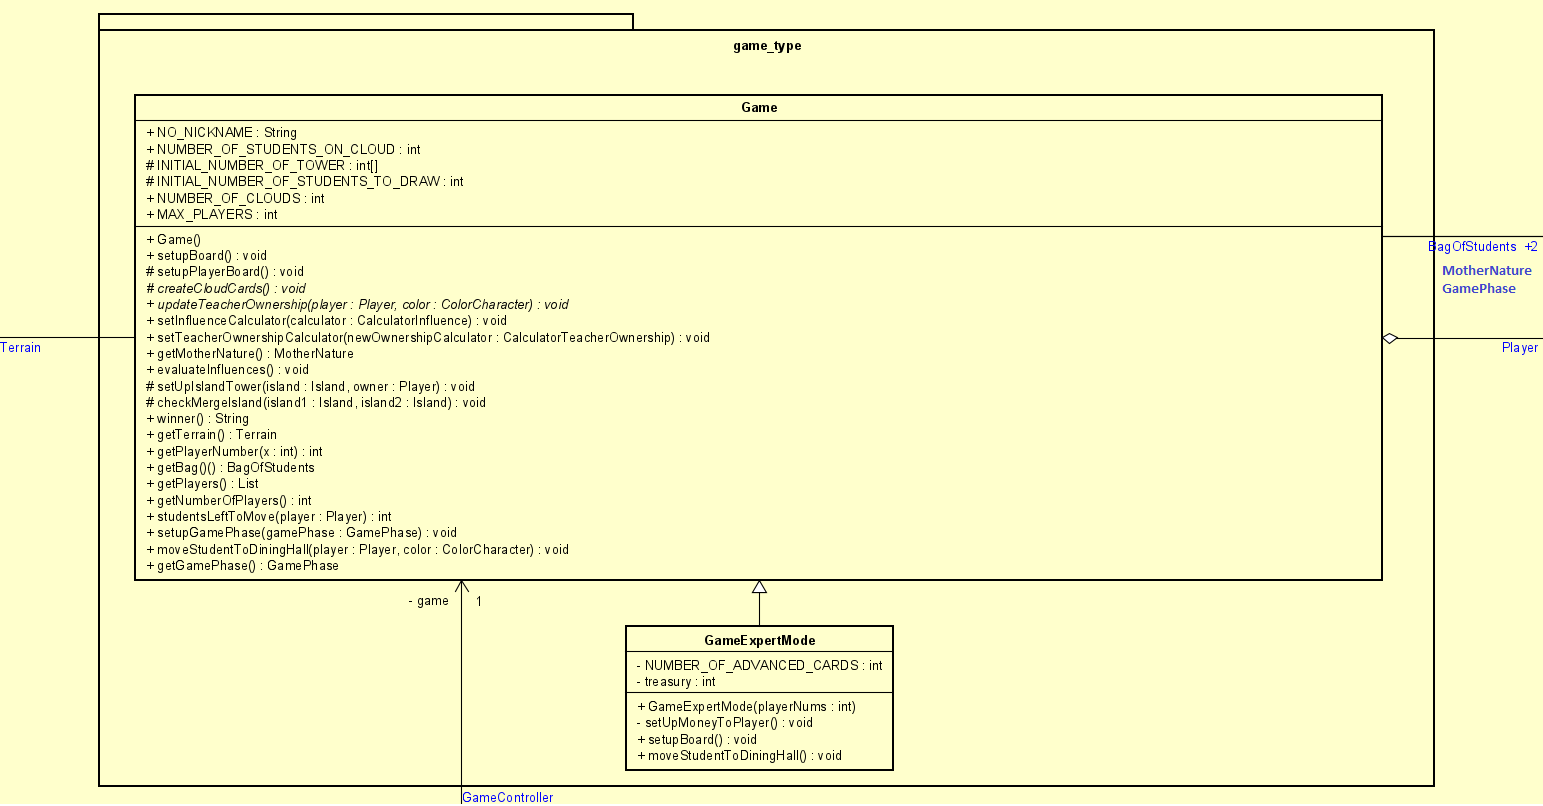
\includegraphics[scale=0.50]{game class.png}
		\caption{Game Class}
	\end{figure}\\
	\paragraph{}
	La classe Game è il fulcro della nostra struttura. Riassumiamo infatti in tale oggetto tutti i componenti del gioco, quali gli oggetti che compongono il terreno (isole, carte nuvola), i giocatori (players), madre natura, il sacchetto di studenti e i calcolatori di influenza e condizioni di possesso dei professori. Il controller si interfaccerà inizialmente con questa classe per accedere agli oggetti del modello da modificare.\\
	Dalla Game class, si dirama GameExpertMode ovvero il gioco in modalità per esperti. Quest'ultima non modifica in modo netto le funzionalità di base del gioco, ma in certi casi le arricchisce. Pertanto, è stato fatto l'override dei metodi che modificano, seppur parzialmente, il comportamento da assumere in talune situazioni.
	\newpage
	\begin{figure}[h!]
		\centering
		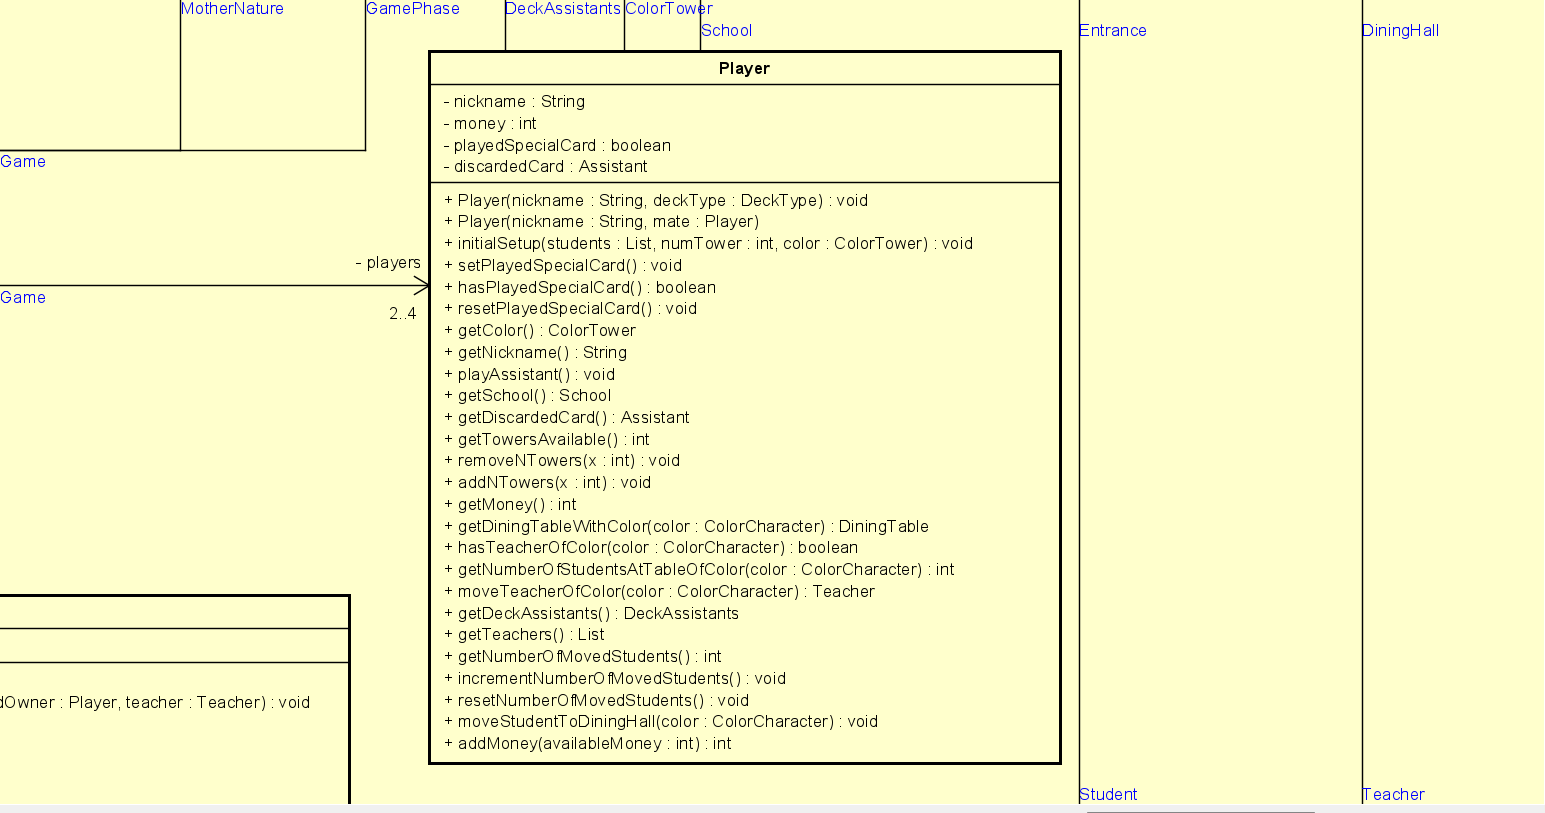
\includegraphics[scale=0.5]{player class.png}
		\caption{Player Class}
	\end{figure}
	\paragraph{}
	La classe player riassume tutte le proprietà di un giocatore, dal suo nickname, al suo mazzo di carte assistente, alla sua plancia di gioco...\\
	Ogni giocatore avrà quindi una corrispettiva rappresentazione all'interno del modello che ne conterrà lo stato per tutto il corso della partita.\\
	\begin{figure}[h!]
		\centering
		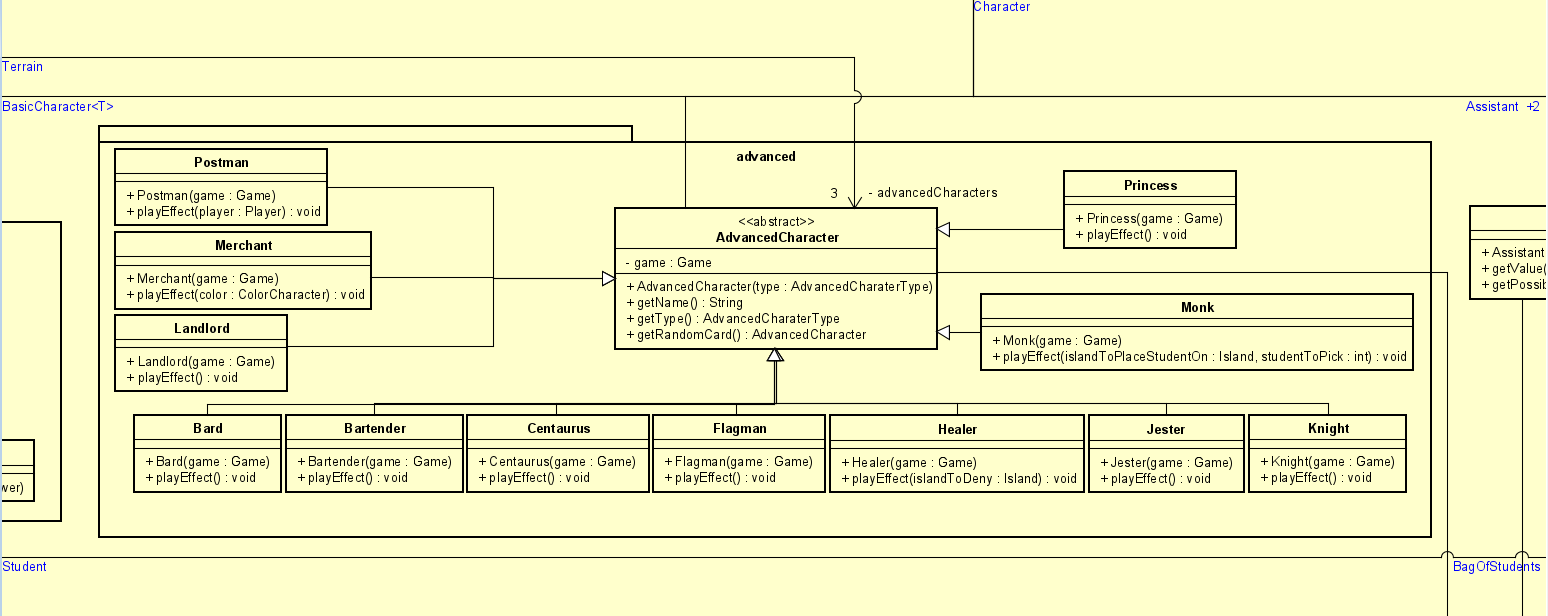
\includegraphics[scale=0.5]{advanced class.png}
		\caption{AdvancedCharacter Class \& Implementazione Personaggi}
	\end{figure}
	\paragraph{}
	La sezione \emph{advanced} contiene le carte personaggio. Come detto in precedenza, per rendere trasparente ed estendibile l'implementazione delle suddette carte, abbiamo deciso di utilizzare una classe per ciascun personaggio. Comune a tutti è la presenza di un riferimento al game in modo tale che il metodo playEffect possa decorare, a seconda della carta, la funzionalità di interesse seguendo la specifica.
	
	\newpage
	\begin{figure}[h!]
		\centering
		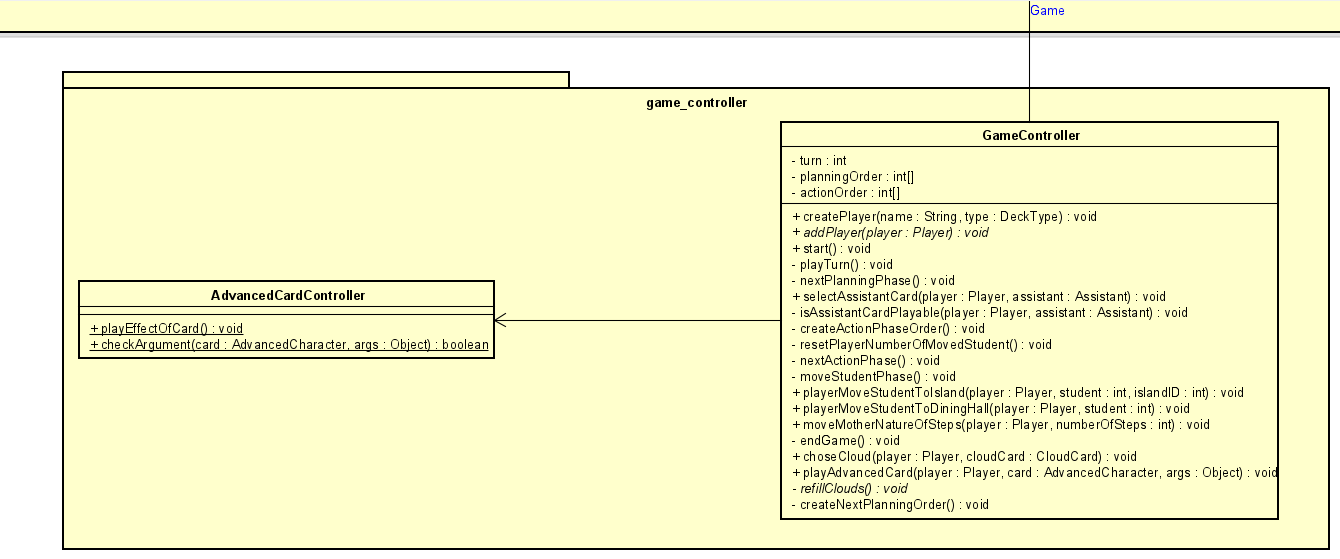
\includegraphics[scale=0.5]{controller.png}
		\caption{Controller}
	\end{figure}
	\paragraph{}
	Riportiamo infine per completezza una breve descrizione dell'idea che ci siamo fatti del controller. Di seguito forniamo una breve descrizione dei metodi principali che \emph{dovrebbero} riassumere i possibili comandi che un giocatore deve poter eseguire (ogni metodo è responsabile di effettuare i controlli sulla fattibilità della mossa richiesta):
	\begin{itemize}
		\item \emph{createPlayer \& addPlayer} rispondono alla volontà del giocatore di iscriversi alla partita in fase di creazione con i parametri indicati;
		\item \emph{start} fa iniziare il match;
		\item \emph{selectAssistantCard} fa giocare al giocatore la carta assistente da lui selezionata;
		\item \emph{playerMoveStudentToIsland} permette al giocatore di muovere lo studente selezionato dal suo ingresso all'isola selezionata;
		\item \emph{playerMoveStudentToDiningHall} permette al giocatore di muovere lo studente selezionato dal suo ingresso alla sua sala;
		\item \emph{moveMotherNatureOfSteps} permette al giocatore di muovere madre natura della quantità di passi indicata (valutazione dell'influenza delle isole, eventuale costruzione di torri e merge di isolotti adiacenti sono operazioni interne triggerate a fine del movimento di madre natura);
		\item \emph{choseCloud} permette al giocatore di prelevare gli studenti dalla cloud card selezionata;
		\item \emph{playAdvancedCard} permette al giocatore di giocare l'effetto della carta personaggio selezionata.
	\end{itemize}
	
	% Week 4: Teting del modello
	\newpage
	\subsection{Settimana 4: Testing del Modello}
	\paragraph{}
	Nella quarta settimana di sviluppo è stata consolidata la struttura del nostro modello analizzando nuovamente l'implementazione delle carte avanzate. Sono inoltre stati testati buona parte dei metodi del Model, come quelli inerenti al calcolo dell'influenza su un'isola, verifica delle condizioni di ownership dei professori, merging di isole adiacenti conquistate da uno stesso giocatore, etc...\\
	Riportiamo di seguito, per completezza, la versione del diagramma UML aggiornata alla quarta settimana:\\
	\begin{figure}[h]
		\centering
		\def\svgwidth{\columnwidth}
		\resizebox{\linewidth}{!}{\input{{umlFourthWeek.pdf_tex}}}
		\caption{Class Diagram - Quarta settimana}
	\end{figure}\\
	
	\paragraph{}
	Infine è stato stilato il documento di Peer-Review del gruppo GC13 (vedi \emph{/Deliverables/Peer Reviews/Peer-Review-1-UML-GC13.pdf}).
	
	% Week 5: controller tests & network arch init
	\newpage
	\subsection{Settimana 5: Controller tests ed architettura di rete}
	\paragraph{}
	Nella quinta settimana di sviluppo sono stati testati i metodi del controller per verificarne il comportamento atteso a valle di test cases standard. Inoltre, in vista dell'introduzione della rete, il controller è stato corredato da diversi oggetti rappresentanti le azioni e richieste che il giocatore vuole eseguire durante una partita.\\
	\begin{figure}[h!]
		\centering
		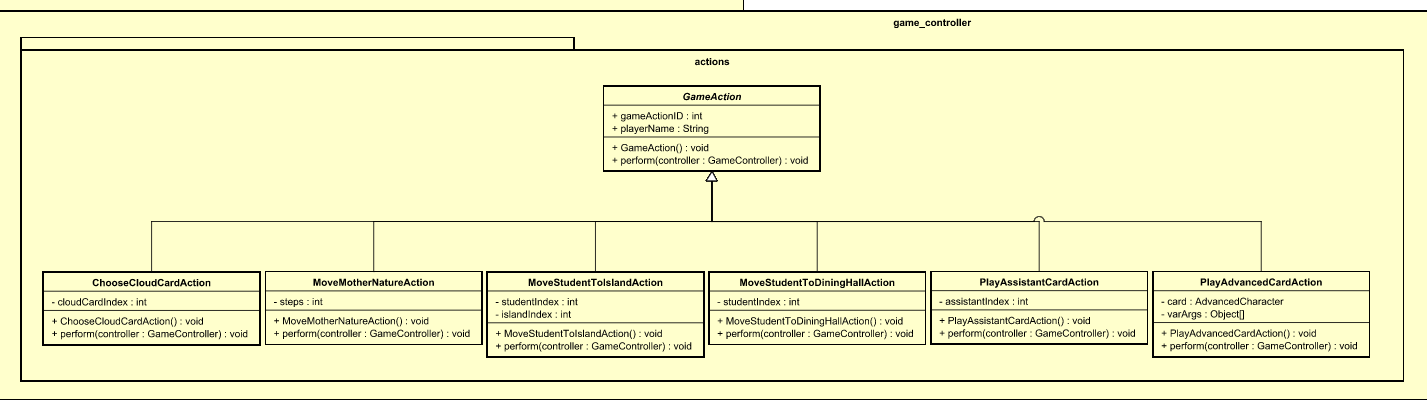
\includegraphics[scale=0.55]{gameActions.png}
		\caption{Controller game actions}
	\end{figure}
	\paragraph{}
	Tali azioni saranno oggetto di scambio tra client e server per gestire l'applicazione di azioni da parte del controller sul modello. Il metodo \textit{perform} di ogni azione, infatti, esegue l'operazione chiamando i rispettivi metodi del controllore con i dovuti parametri.\\
	Infine, a seguito dell'esercitazione svolta su \emph{Socket e Serializzazione} è stata inserita una prima versione dell'architettura di rete.
	
	% Week 6: Network & CLI initialization
	\newpage
	\subsection{Settimana 6: Network multi-partita e CLI}
	\paragraph{}
	Nel corso della sesta settimana di sviluppo abbiamo parallelamente aggiornato la nostra struttura di rete ed implementato un'iniziale versione di interfaccia utente da linea di comando.\\
	\begin{figure}[h]
		\centering
		\def\svgwidth{\columnwidth}
		\resizebox{\linewidth}{!}{\input{{umlFifth&SixthWeek.pdf_tex}}}
		\caption{Class Diagram - Quinta e Sesta settimana}
	\end{figure}
	\paragraph{}
	Siamo pertanto riusciti a testare la nostra implementazione fino a poter giocare una partita completa con le regole standard. Di seguito riportiamo un elenco delle attività svolte:\\
	\begin{itemize}
		\item Interfaccia grafica da linea di comando. Abbiamo creato delle \textit{micro-classi} con lo scopo di rappresentare i vari componenti fisici del gioco. Queste rispetto al modello si distinguono per essere in minor numero (attualmente sono 6) e per contenere solo i dati essenziali a rappresentare la board in maniera visiva. Inoltre queste classi fanno override del metodo \textit{toString} così facendo viene automatico stampare sulla CLI un update grafico del gioco. La CLI fa uso di codici di escape ANSI per gestire i colori.
		\item Implementazione della funzionalità avanzata "Partite Multiple" attraverso un sistema di gestione a Lobby .
		\item I messaggi scambiati tra Client e Server sono tutti degli oggetti della classe \textit{CommunicationMessage} così facendo abbiamo un solo tipo di messaggio che viene scambiato e la comunicazione risulta più semplice. in base ad un ID sappiamo se il contenuto contiene un update grafico della board, azioni richieste dal client e altri ancora. Tra le azioni richiesta da client risultano le classi create la scorsa settimana \textit{GameActions} che vengono poi eseguite dal server.
	\end{itemize}

	% Week 7: Disconnessioni, completamento interfaccia CLI e inizio interfaccia GUI
	\newpage
	\subsection{Settimana 7: Disconnessioni, completamento interfaccia CLI e inizio interfaccia GUI}
	\paragraph{}
	Nel corso della settima settimana di sviluppo abbiamo controllato e sistemato come si comportava il server a seguito di una disconnessione lato client, completato l'implementazione dell'interfaccia cli (ad eccezione di come vengono raccolti i dati richiesti da alcune carte avanzate) e adattato ed iniziato il client per poter essere eseguito in modalità GUI\\
	 
	\begin{itemize}
		\item \textbf{Disconnessioni del client:} abbiamo deciso di raggruppare il più possibile le eccezioni che potevano essere lanciate dal server (per quanto riguarda la parte del codice che si occupa di rispondere alle richieste del client) in modo da dover gestire le disconnessioni solo in due luoghi.
		\item \textbf{Ping system:} per gestire l'eventualità in cui un giocatore perda la connessione, è stato introdotto un ping system lato server, il quale ogni 10 secondi invia per l'appunto un \textit{CommunicationMessage} di tipo ping. La risposta del client a questo genere di messaggi è generalmente immediata (in condizioni normali servono pochi millisecondi); tuttavia in caso di caduta di connessione se il server non riceve un \textit{CommunicationMessage} di tipo pong entro 10 secondi, chiude la connessione decretando l'effettiva perdita di collegamento con il client.
		\item \textbf{Logger:} è stata implementata una classe \textit{Logger} che permette di mostrare in console messaggi formattati per avere un riscontro su ciò che sta accadendo \textit{'dietro le quinte'}. Al momento sono distinti le seguenti tipologie di messaggio: \textit{ERROR, INFO, GAME\_LOG, WARNING}.
		\item \textbf{Completamento interfaccia CLI:} abbiamo completato l'interfaccia da linea di comando, tra le modifiche più essenziali risulta esserci quella della gestione del client con una macchina a stati, ciò ci permette di avere un unico punto in cui leggere i messaggi dal socket con il server. Così facendo quando il server risponde, che sia un aggiornamento della partita o un errore, siamo sicuri che la lettura avvenga una sola volta e che venga eseguita l'azione corretta.
		\item \textbf{Implementazione GUI:} oltre al resto abbiamo cominciato a sviluppare la GUI, per fare ciò ed avere le stesse azioni della CLI (ma con implementazioni diverse) abbiamo creato un interfaccia. 
		Per leggere i messaggi che arrivano al client è stata creata una classe che fa da Observer per i messaggi e poi chiama il metodo dell'interfaccia (interpellata sopra) in modo da poter aggiornare anche la CLI in una maniera che ci sembra più pulita e ordinata e permette un implementazione di nuove azioni in maniera facile e lineare sia per CLI sia per GUI. 
		È stata stesa una prima pagina della GUI per la fase iniziale.\\
	\end{itemize}
	\newpage
	\begin{figure}[h!]
		\centering
		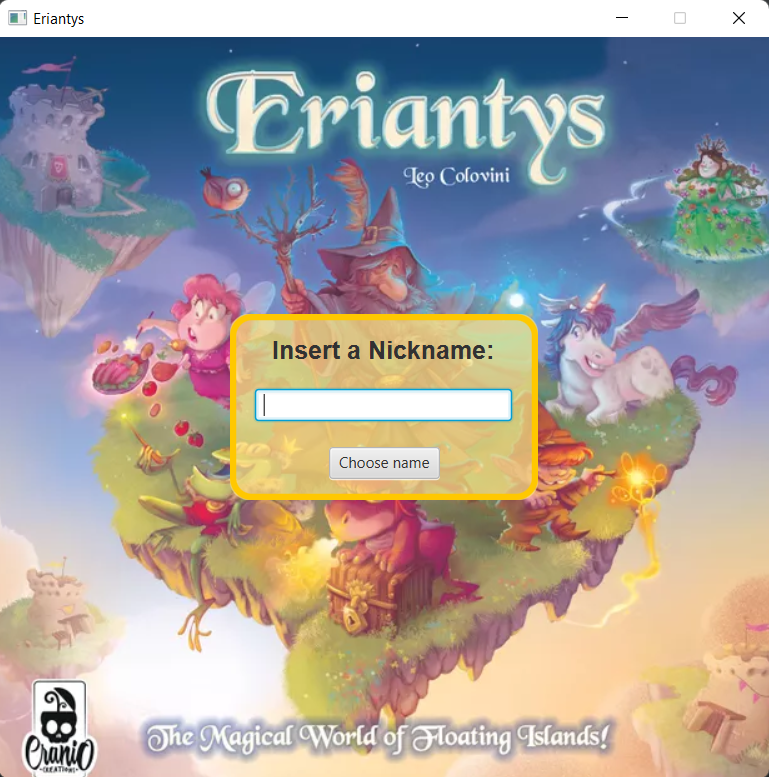
\includegraphics[scale=0.45]{first_GUI_page.png}
		\caption{First GUI page :D}
	\end{figure}
	Per completezza, riportiamo il Class Diagram aggiornato:\\
	\begin{figure}[h!]
		\centering
		\def\svgwidth{\columnwidth}
		\resizebox{\linewidth}{!}{\input{{umlSeventhWeek.pdf_tex}}}
		\caption{Class Diagram - Settima settimana}
	\end{figure}\\
	
	\paragraph{}
	Alleghiamo infine un \textit{sequence diagram} che riassume la fase di connessione di un player al server, dalla creazione del suo \textit{socket}, alla costruzione di una nuova partita o partecipazione ad una lobby già esistente, fino al momento di inizio effettivo della partita stessa:\\
	\newpage
	\begin{figure}[h!]
		\centering
		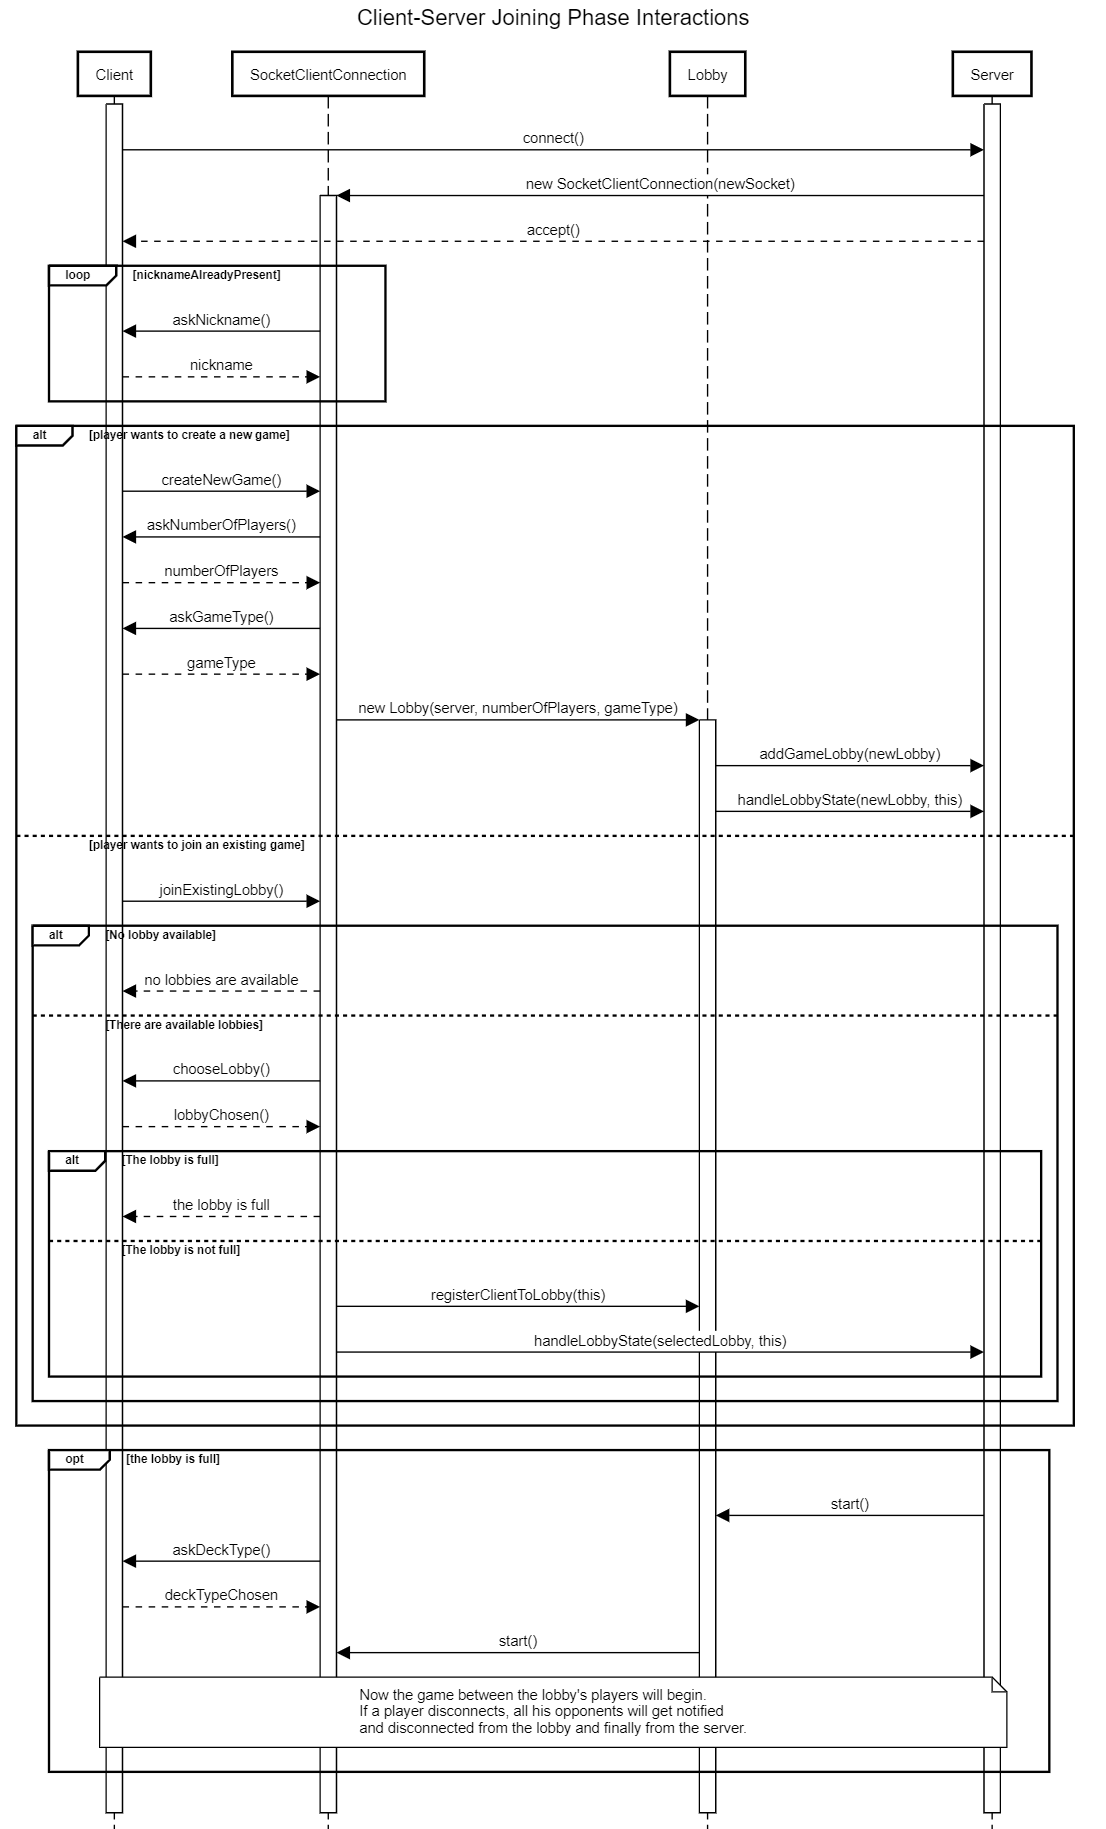
\includegraphics[scale=0.33]{SequenceDiagramJoiningPhaseInteractions.png}
		\caption{Sequence Diagram - Connessione al server e primi passi}
	\end{figure}
	
	\newpage
	% Week 8: enhanced gui, extended ping system, server passive
	\subsection{Settimana 8: Miglioramenti CLI\&GUI, Ping System esteso, server passivo}
	\paragraph{}
	Nell'ottava settimana di sviluppo sono stati fatti significativi passi avanti per quanto riguarda il reparto grafico e di interfaccia utente. Inoltre è stato esteso il ping system lato client in modo tale che anche l'applicativo client-side possa accorgersi di eventuali cadute di connessione del server. Infine, sono stati analizzati i documenti in preparazione alla peer review sull'architettura di rete.
	\paragraph{}
	La struttura del network è stata consolidata; sia server sia client riescono a reagire ad eventuali perdite di connessione dell'una o dell'altra parte, terminando il loro processo come da specifica.\\
	\begin{figure}[h!]
		\centering
		\def\svgwidth{\columnwidth}
		\resizebox{\linewidth}{!}{\input{{umlEightWeek.pdf_tex}}}
		\caption{Class Diagram - Ottava settimana}
	\end{figure}\\
	\paragraph{}
	Abbiamo inoltre modificato il comportamento del server in fase di setup di connessione. Nella settimana precedente, il server in tale frazione si comportava da componente attivo. Nel corso della settimana corrente è stata invertita la logica.
	\paragraph{}
	Riportiamo dunque alcuni sequence diagram che riteniamo significativi.
	Il primo rappresenta la fase di connessione del client al server fino all'effettivo join di una lobby, che sia creata dal player stesso o che sia di un altro giocatore. Il secondo mostra il funzionamento del ping system, mentre l'ultimo illustra una generica azione di gioco.
	
	\newpage
	\begin{figure}[h!]
		\centering
		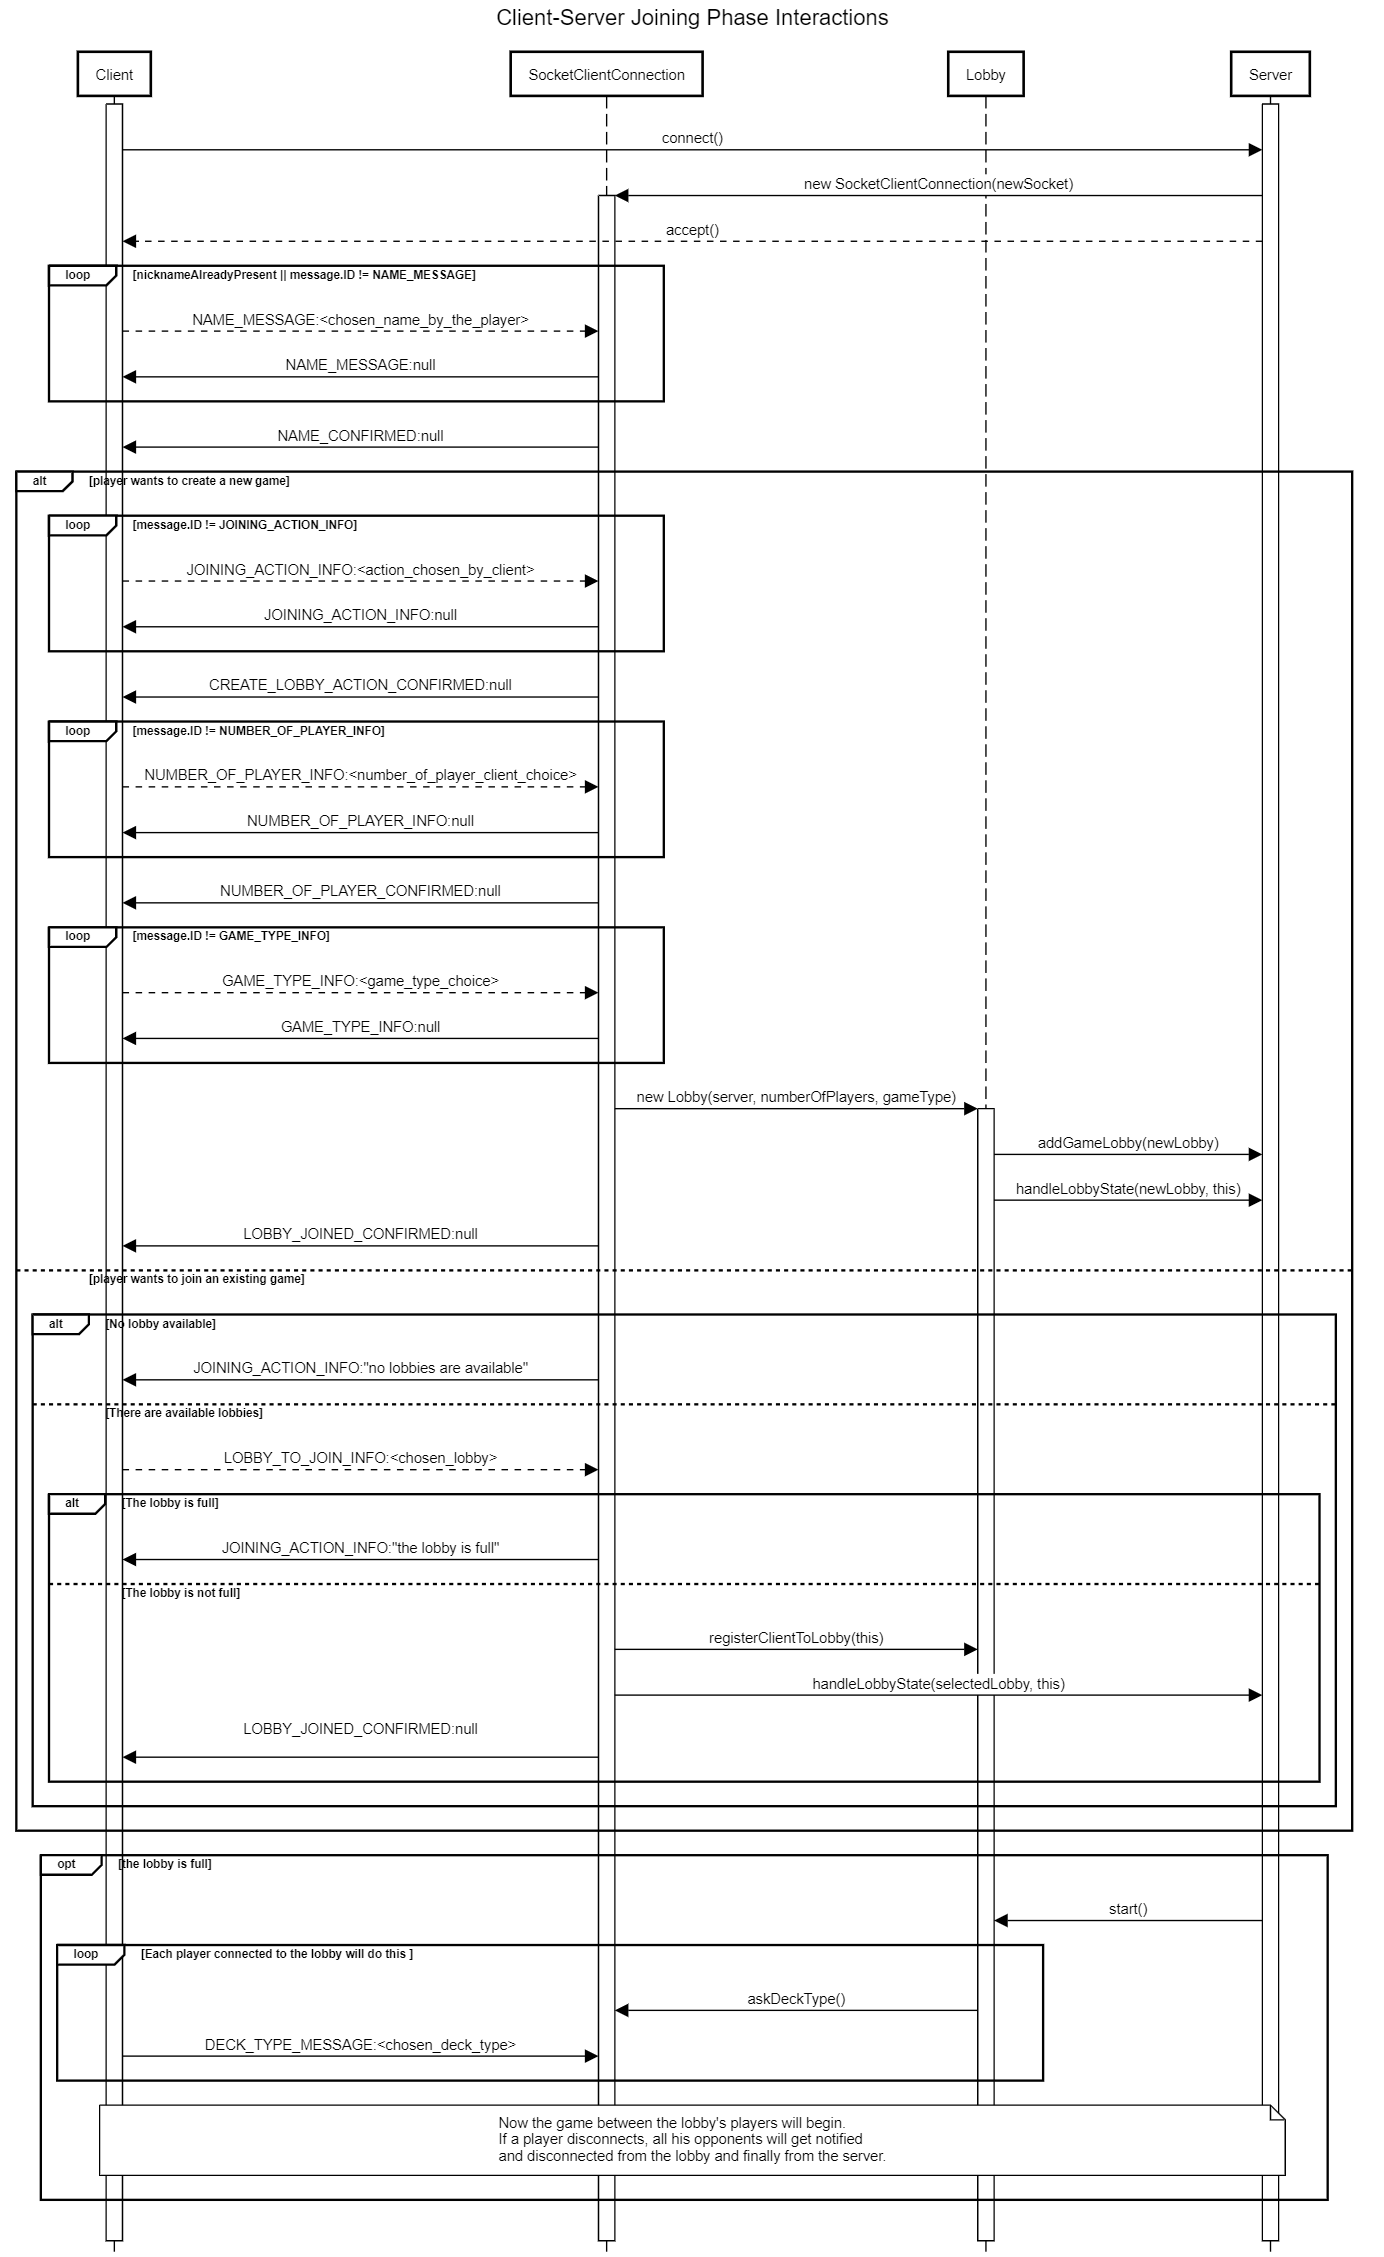
\includegraphics[scale=0.27]{ClientServerJoiningPhaseInteraction1.png}
		\caption{Sequence Diagram - Connessione al server aggiornato}
		\label{fig:sequence_join}
	\end{figure}
	\newpage
	\begin{figure}[h!]
		\centering
		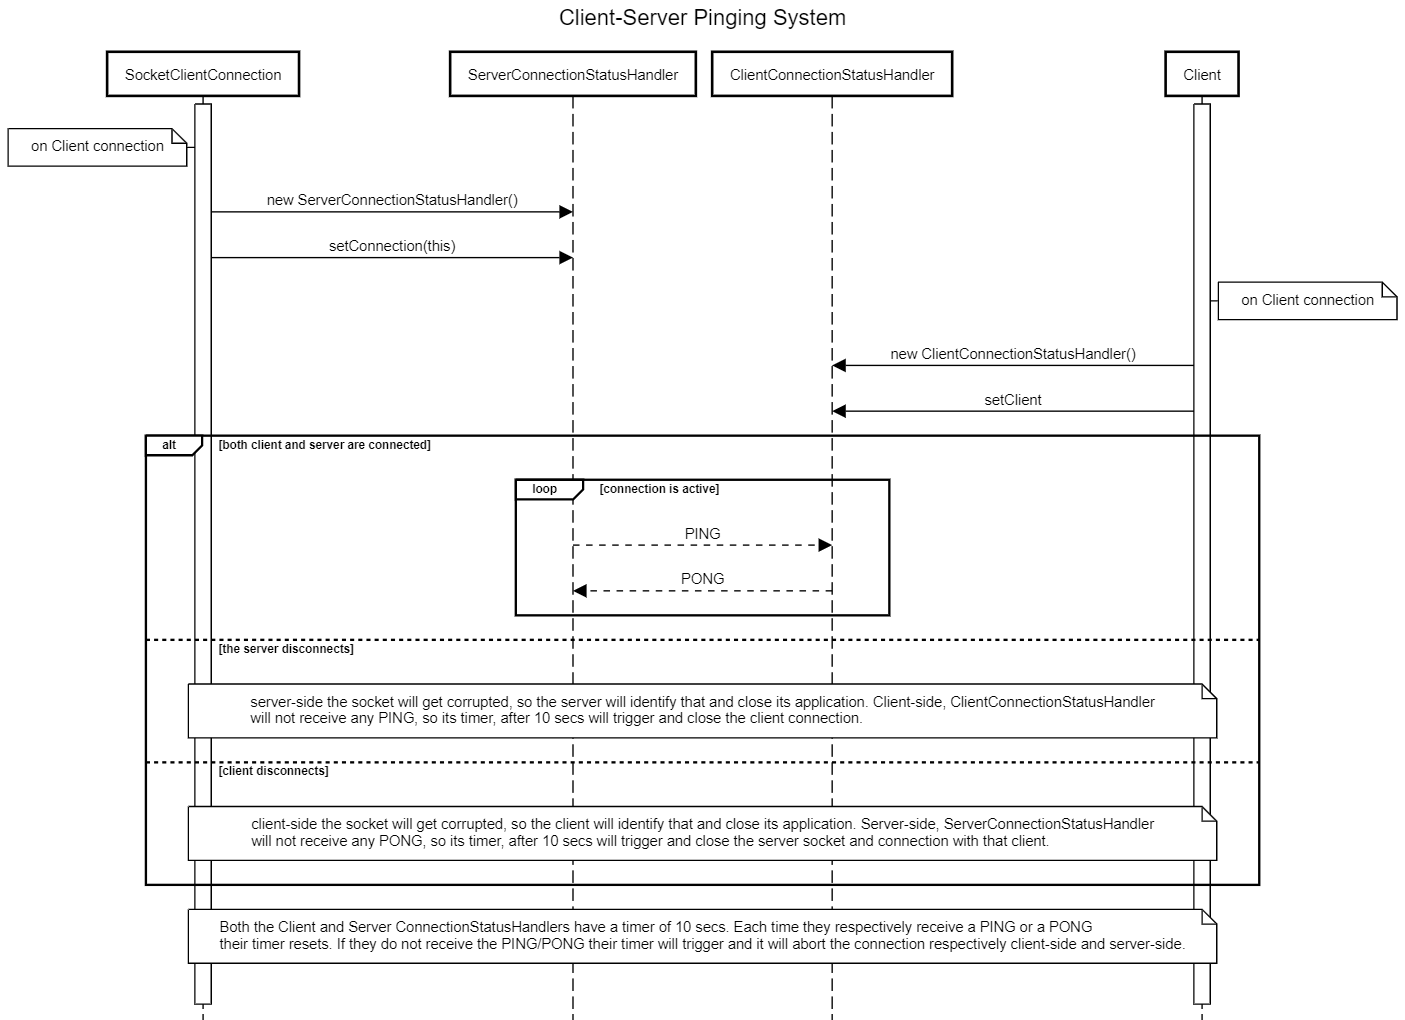
\includegraphics[scale=0.3]{PingingSystem.png}
		\caption{Sequence Diagram - Ping Pong}
		\label{fig:sequence_pingpong}
	\end{figure}
	\begin{figure}[h!]
		\centering
		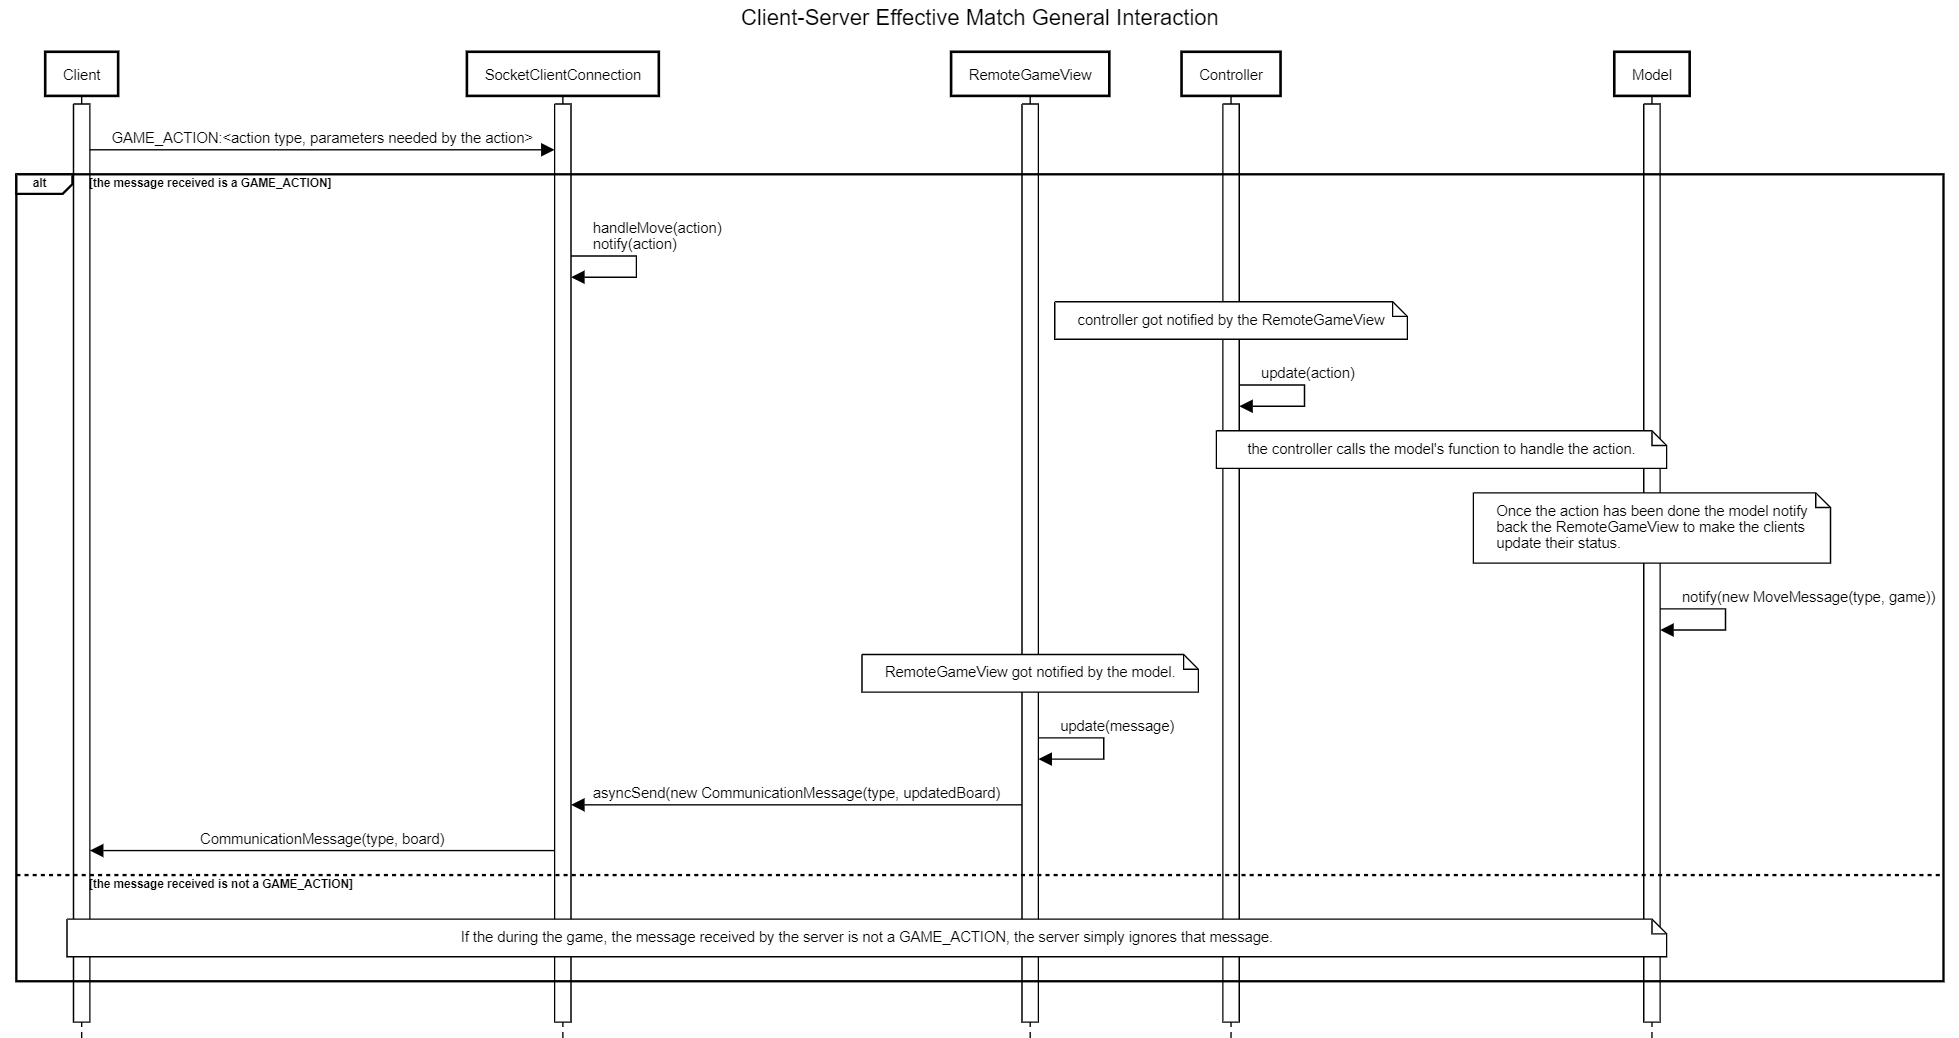
\includegraphics[scale=0.25]{ClientServerEffectiveMatchGeneralInteraction.png}
		\caption{Sequence Diagram - General Move Message}
		\label{fig:sequence_generalmove}
	\end{figure}

	\newpage
	\subsubsection{Peer Review - Network}
	\paragraph{}
	In vista dell'attività di \textbf{peer review} della nona settimana di sviluppo, riportiamo i componenti dell'ambiente di network.\\
	\begin{figure}[h!]
		\centering
		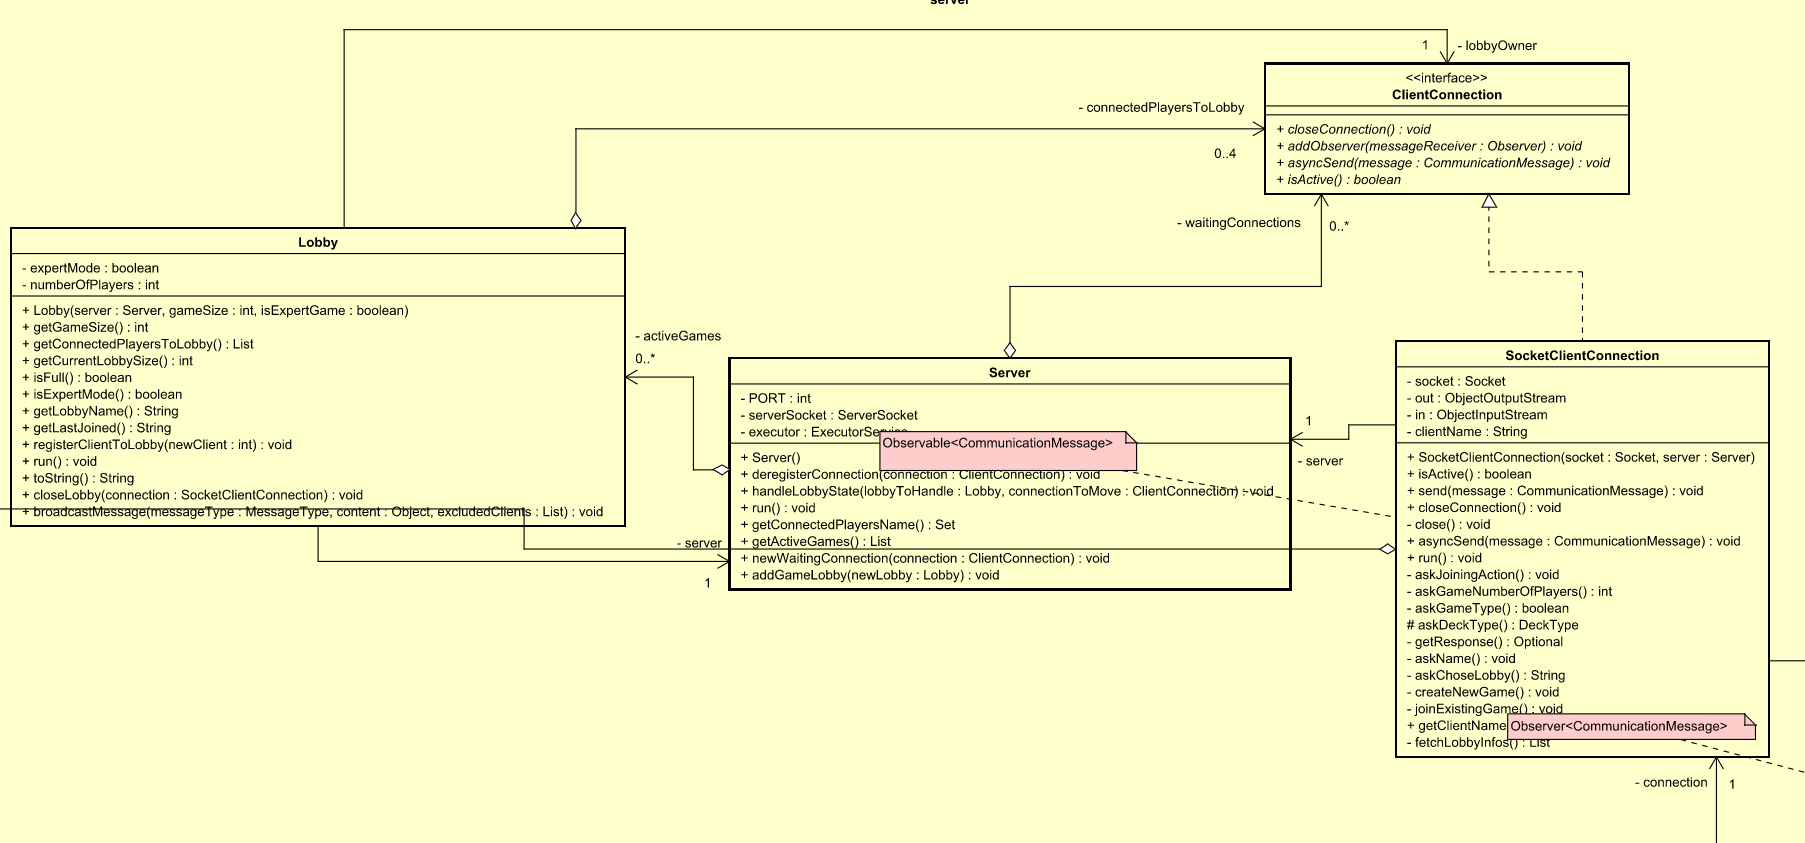
\includegraphics[scale=0.45]{serverSideArch.png}
		\caption{Architettura Server Side}
	\end{figure}\\
	\begin{itemize}
		\item Alla connessione di un client, il server la accetta consolidando il socket per la comunicazione. Quest'ultimo verrà gestito dall'oggetto \textit{SocketClientConnection}.
		\item Per implementare la funzionalità aggiuntiva \textit{Partite Multiple} abbiamo creato un sistema a lobby. Ogni oggetto \textit{Lobby} gestisce una singola partita. Un giocatore, una volta entrato nel server e settato il proprio nickname, può scegliere se creare una nuova lobby o entrare in una già esistente (se presente e non piena). Il giocatore che crea la lobby imposta in fase di creazione i parametri della partita stessa.
		\item All'interno della \textit{SocketClientConnection} sono presenti tutte le funzioni che gestiscono le fasi che intercorrono dalla connessione del player al server fino al suo effettivo join in una partita. (settaggio nickname, creazione o join di una lobby, richiesta del tipo di deck da usare nella partita in fase di avvio (Mago, Saggio, Fata, Re)).
		\item i nickname dei player sono unici per tutta la durata della connessione di un client al server. Pertanto anche tra partite differenti non sarà possibile avrà 2 giocatori con lo stesso nick.
		\item il metodo deregister connection gestisce la disconnessione di un client al server. Se il client è parte di una lobby, quest'ultima viene chiusa e tutti i client al suo interno disconnessi.
	\end{itemize}
	
	\newpage
	\begin{figure}[h!]
		\centering
		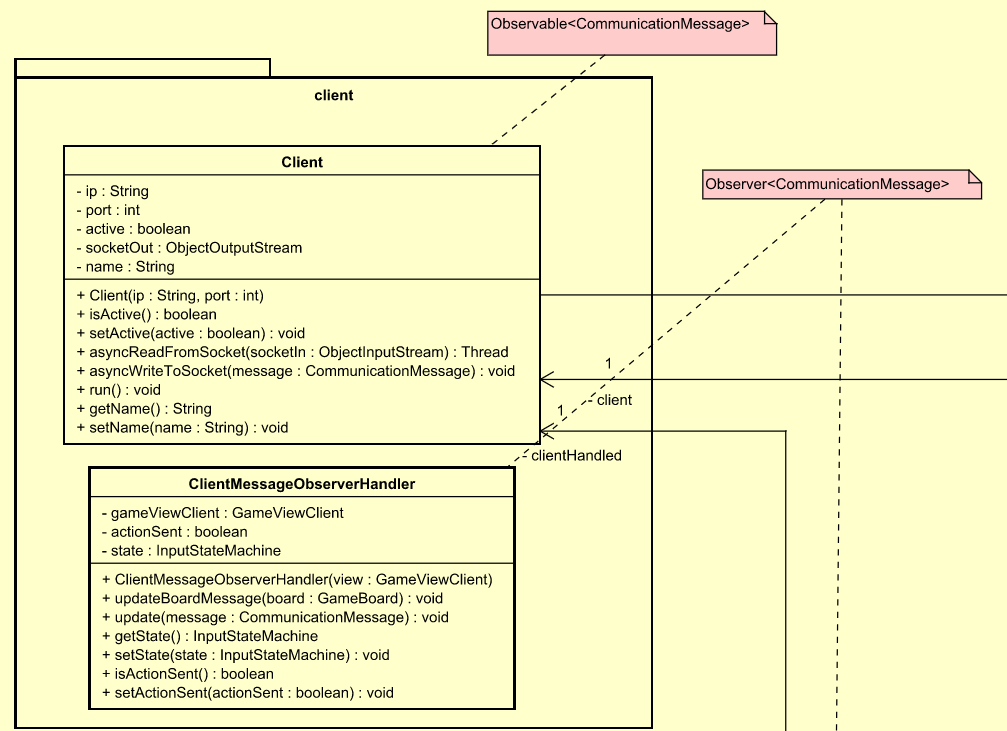
\includegraphics[scale=0.45]{clientSideArch.png}
		\caption{Architettura Client Side}
	\end{figure}
	\begin{itemize}
		\item Il client non appena connesso, viene collegato ad un'istanza dell'oggetto \textit{Client} che gestisce la sua connessione e socket con il server.
		\item L'oggetto \textit{ClientMessageObserverHandler} raggruppa la logica di ricezione dei messaggi (tranne i ping che sono gestiti separatamente). Alla ricezione di un messaggio, in base al suo tipo, un'azione sulla view verrà eseguita.
	\end{itemize}
	
	\begin{figure}[h!]
		\centering
		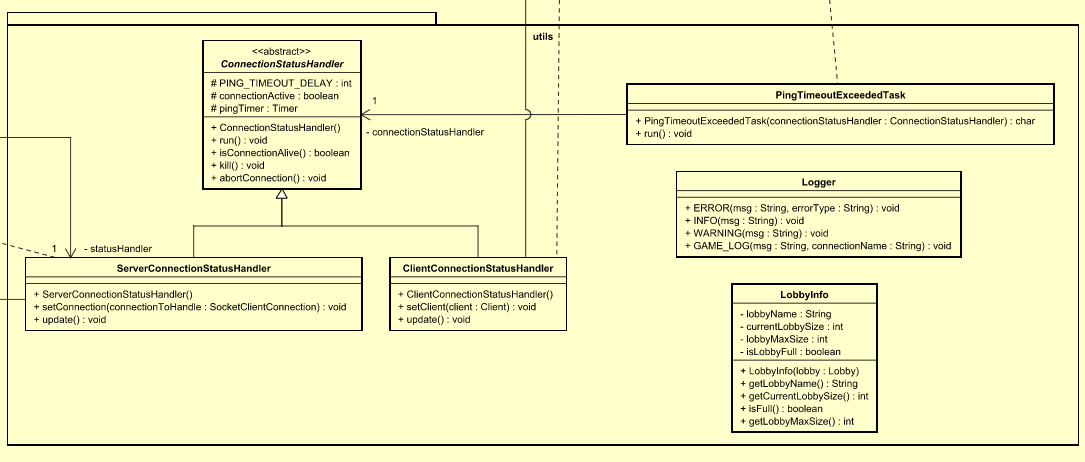
\includegraphics[scale=0.7]{networkUtils.png}
		\caption{Network utilities}
	\end{figure}
	\begin{itemize}
		\item Quando una connessione avviene, come abbiamo detto precedentemente, \textit{SocketClientConnection} e \textit{Client} sono creati rispettivamente su Server e Client. Durante la creazione di questi ultimi, vengono istanziati due nuovi oggetti, rispettivamente \textit{ServerConnectionStatusHandler} e \textit{ClientConnectionStatusHandler}, che gestiscono la connettività ed eventuali problematiche ad essa correlate (perdite di connessione, ragequit, etc...). Il \textit{ServerConnectionStatusHandler} invia periodicamente (default ogni 10 secondi) un messaggio di \textit{PING} al \textit{ClientConnectionStatusHandler} il quale alla ricezione resetta il suo timer e risponde con un \textit{PONG}. Alla ricezione del \textit{PONG} il \textit{ServerConnectionStatusHandler} resetta a sua volta il timer. \cite{javaUtilTimer}
		\item I due timer sono impostati a 10 secondi ciascuno (si ipotizza che in condizioni normali lo scambio ping/pong avvenga in pochi ms). In caso di scadenza di tale timer, viene invocata la task \textit{PingTimeoutExceededTask} che chiude la connessione.
		\item La classe Logger formatta le stringhe e le stampa a schermo aggiungendo una tag colorata in base al tipo di messaggio.
		\item LobbyInfo è un oggetto serializzabile contenente informazioni riguardo una lobby (nome, dimensione massima, dimensione corrente).
	\end{itemize}
	\begin{figure}[h!]
		\centering
		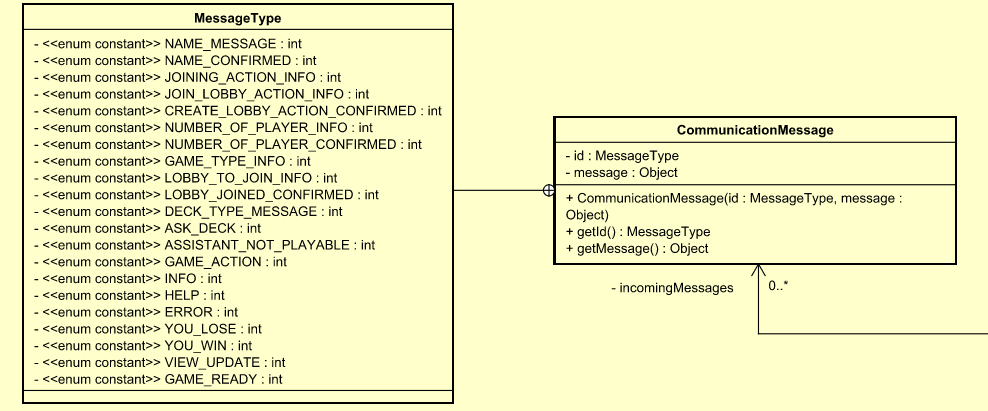
\includegraphics[scale=0.7]{communicationMessage.png}
		\caption{Messaggio di comunicazione}
	\end{figure}
	\begin{itemize}
		\item Oggetto rappresentante i messaggi scambiati tra client e server.
	\end{itemize}
	\paragraph{}
	Per ulteriori informazioni riguardo lo scambio di messaggi, osservare i diagrammi riportati nelle Figure [\ref{fig:sequence_join}][\ref{fig:sequence_pingpong}][\ref{fig:sequence_generalmove}].
	\subsubsection{GUI - Game Board}
	\paragraph{}
	Abbiamo infine implementato una prima versione della Game Board lato GUI:\\
	\begin{figure}[h!]
		\centering
		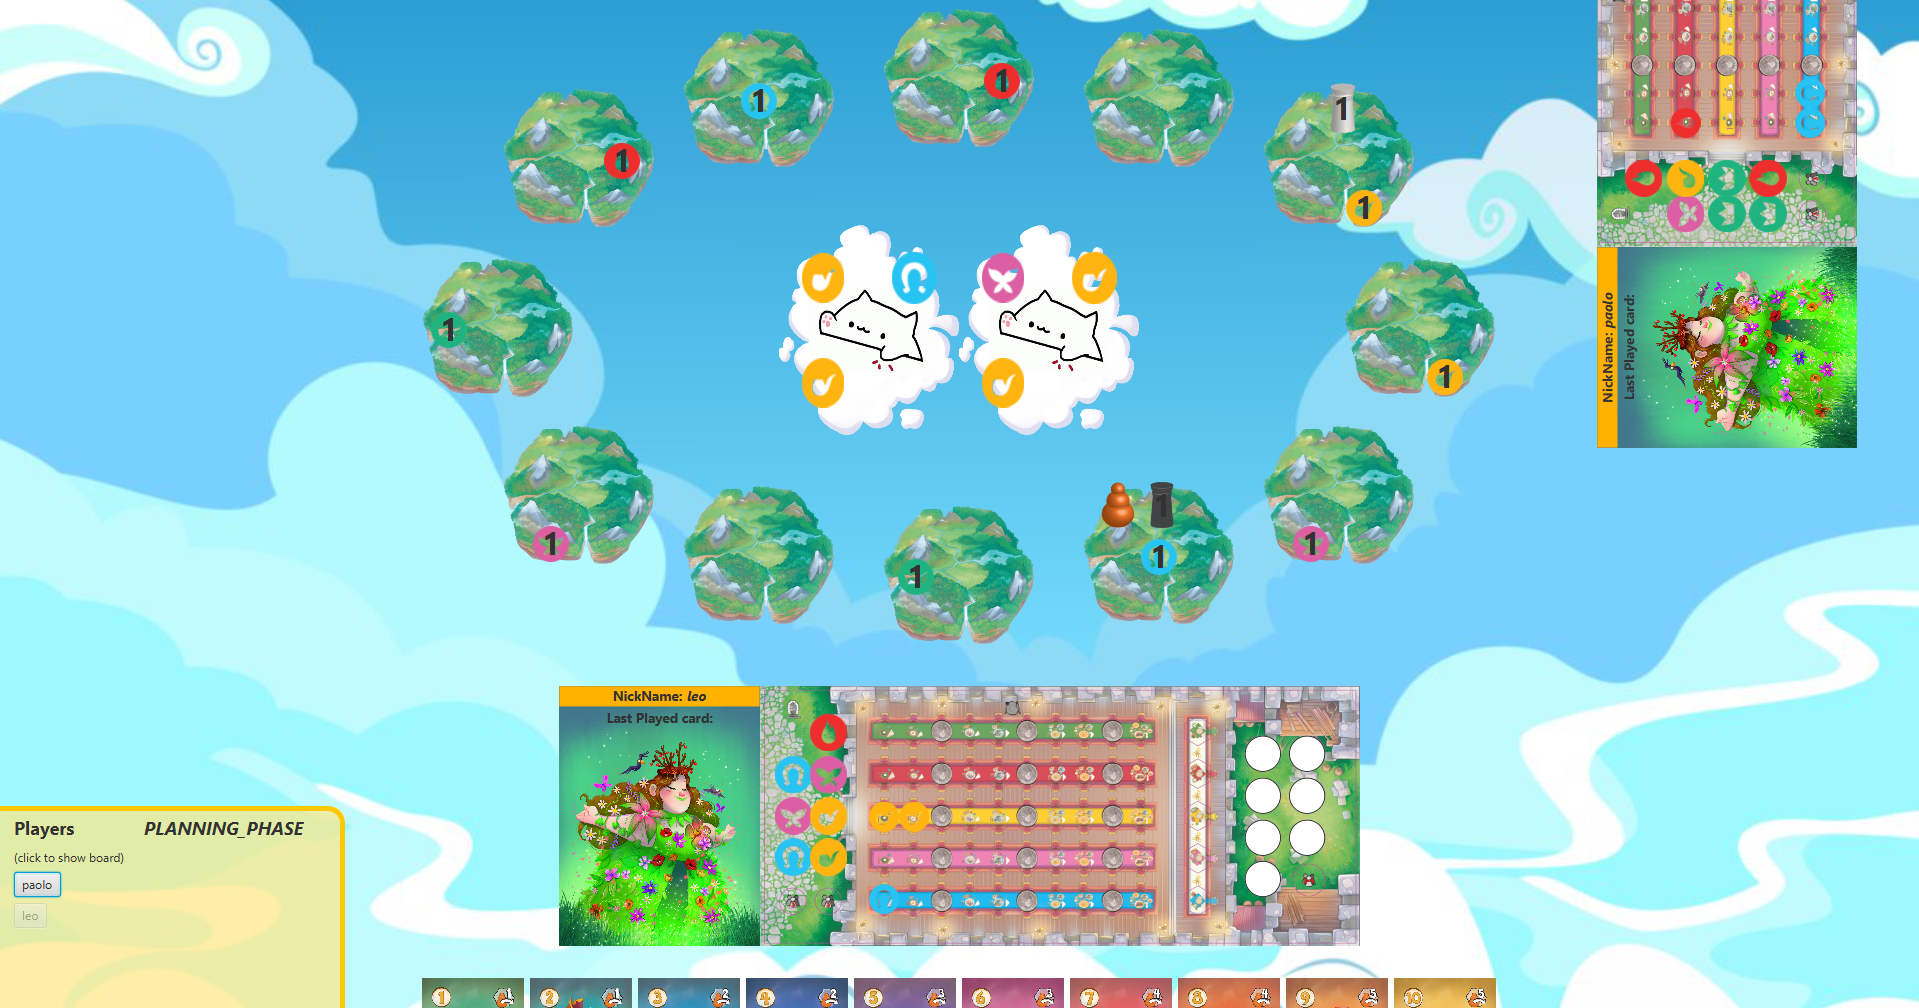
\includegraphics[scale=0.2]{guiGameBoard.png}
		\caption{GUI Game Board}
	\end{figure}
	
	\newpage
	\subsection{Settimana 9: Carte personaggio ed Input handling}
	\paragraph{}
	Nel corso della nona settimana di sviluppo è stata completata una prima versione del gioco. Sono infatti stati ultimate la gestione dell'azione di gioco relativa alle carte avanzate sia lato CLI sia GUI. Al momento \textbf{è} dunque \textbf{possibile effettuare} dall'inizio alla fine \textbf{una partita con regole per esperti per 2 o 3 giocatori}.\\
	Abbiamo inoltre irrobustito la struttura del controller (quindi lato server) per gestire eventuali azioni affettuate da \textit{Malicious Clients}.
	\paragraph{}
	Nelle successive settimane il gruppo si focalizzerà nel testing delle partite a 4 giocatori per completare conseguire con successo il completamento dell'intero progetto con le 3 funzionalità aggiuntive previste.\\
	Riportiamo di seguito due immagini rappresentanti la CLI e la GUI allo stato attuale:
	\begin{figure}[!htb]
		\begin{minipage}{0.495\textwidth}
			\centering
			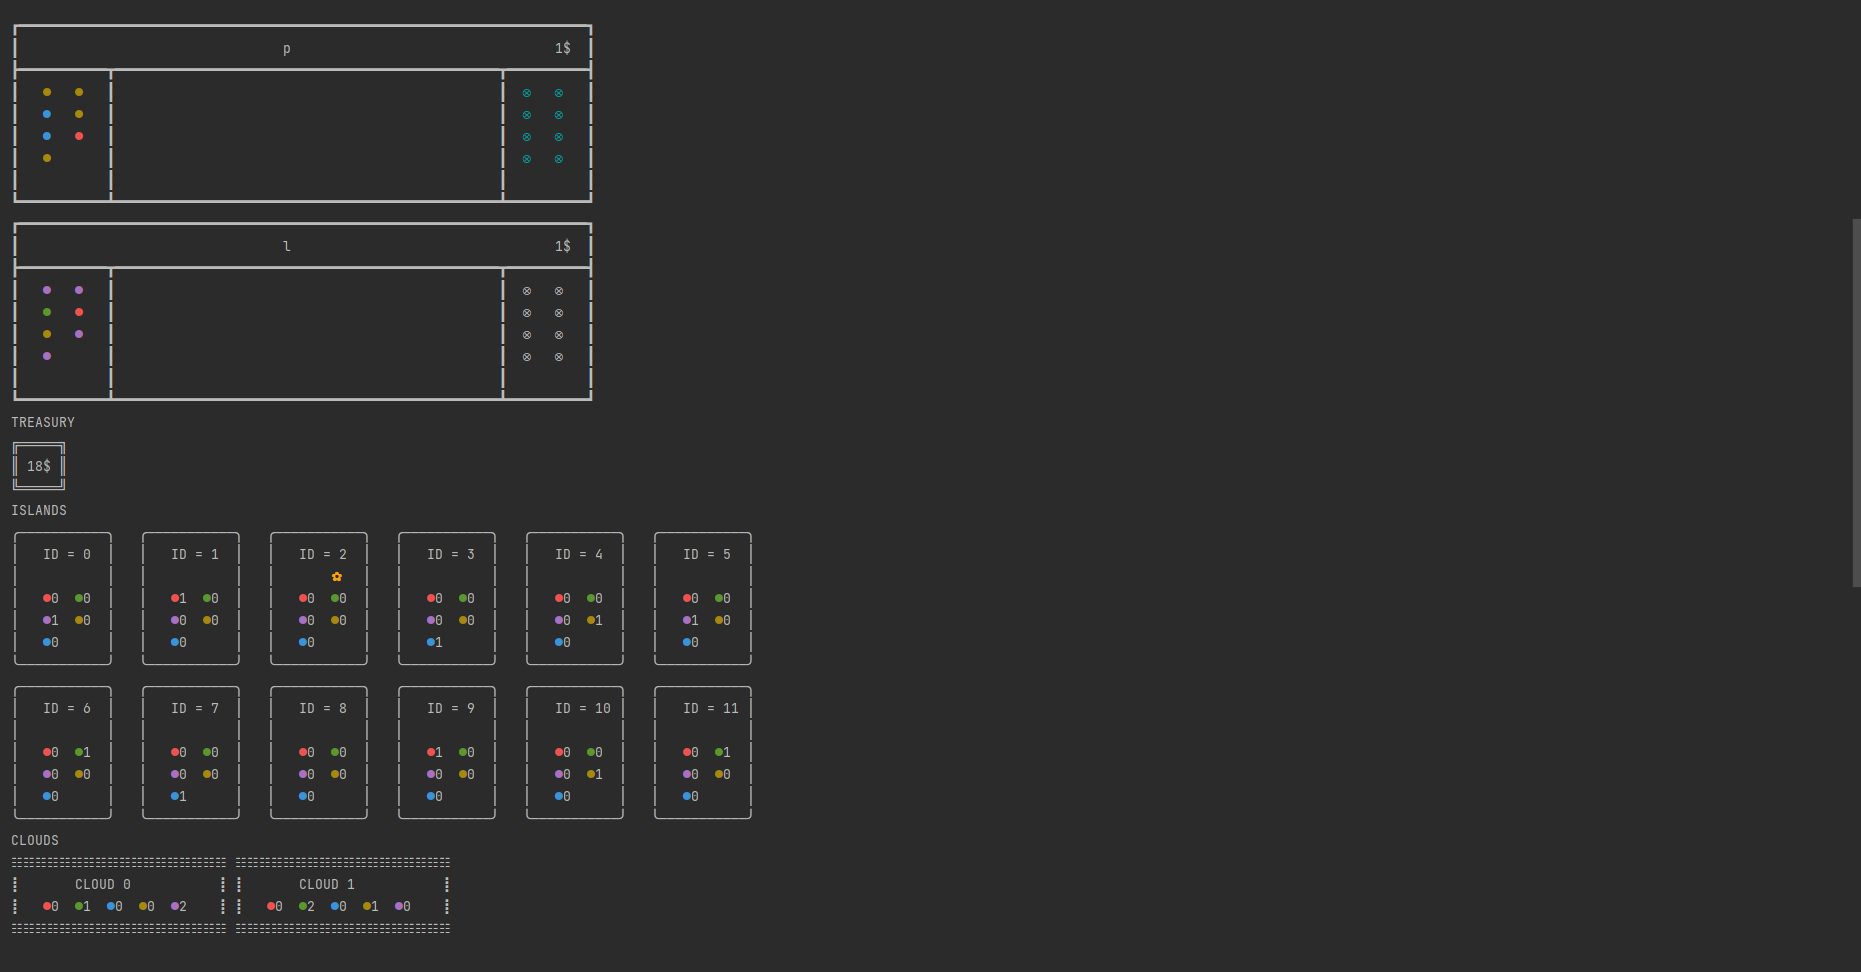
\includegraphics[width=\linewidth]{cliWeek9.png}
			\caption{CLI Player Board \& Islands}
		\end{minipage}\hfill
		\begin{minipage}{0.495\textwidth}
			\centering
			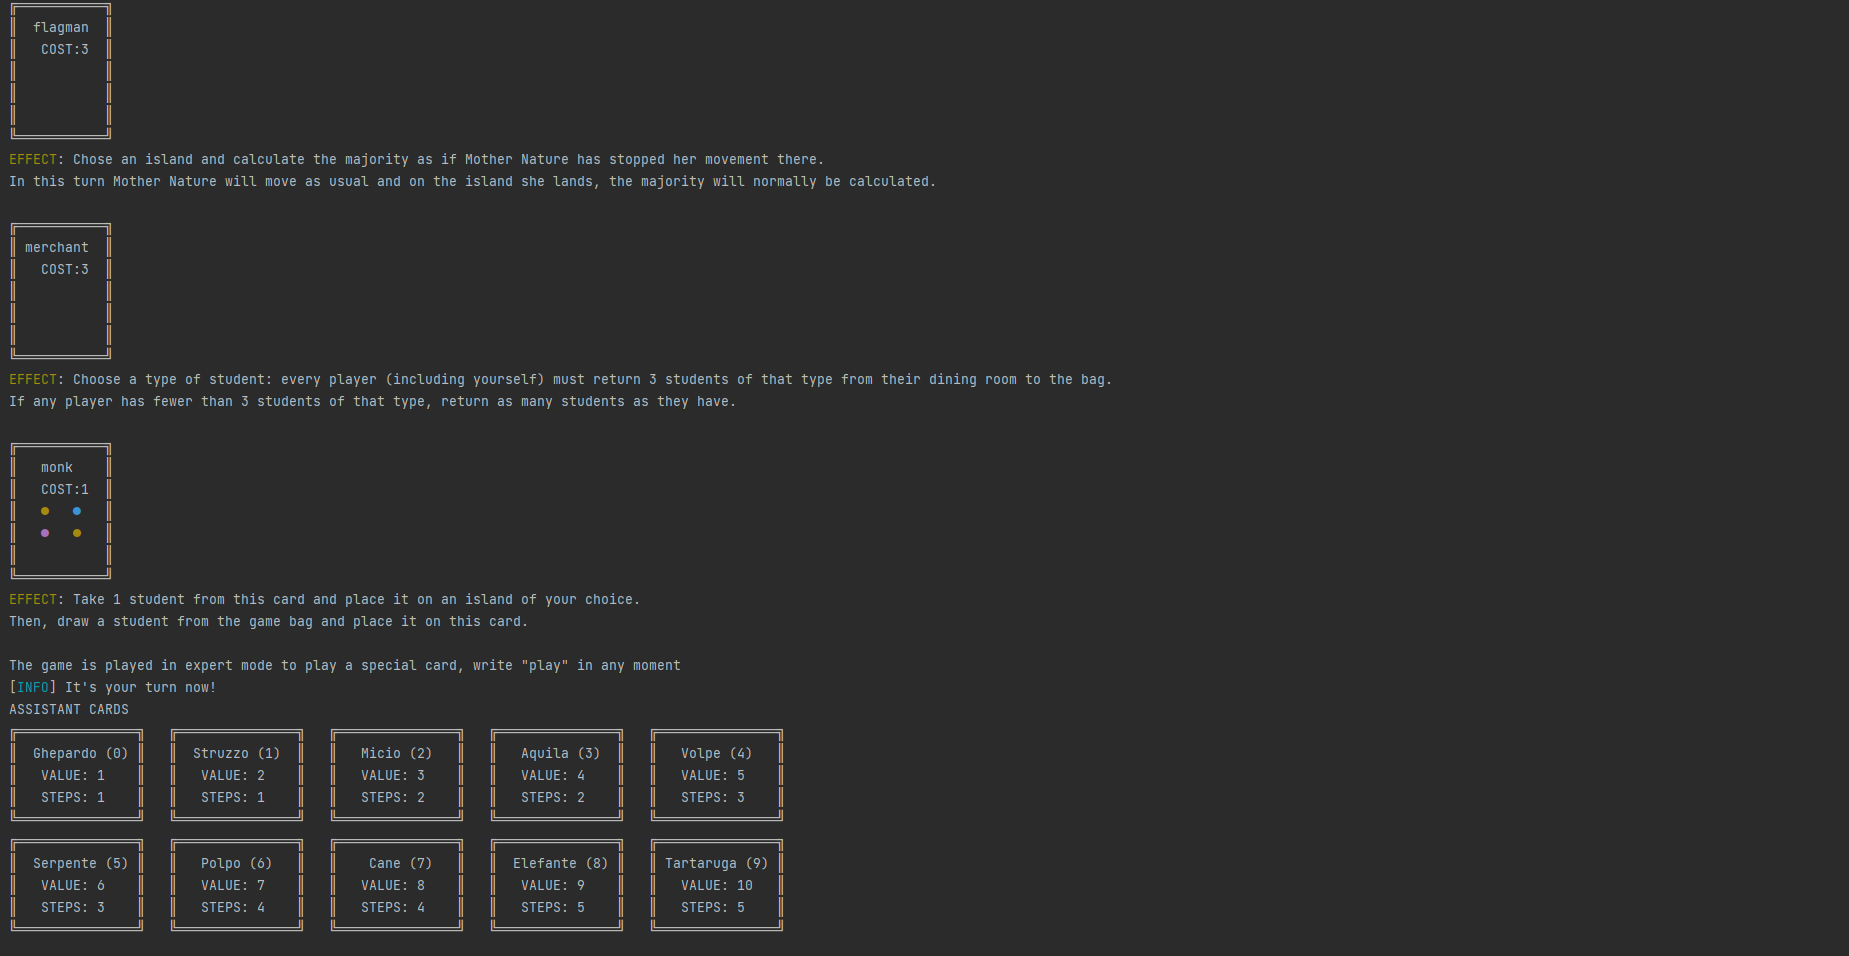
\includegraphics[width=\linewidth]{cli2Week9.png}
			\caption{CLI Carte personaggio / assistente}
		\end{minipage}
	\end{figure}
	\begin{figure}[!htb]
		\begin{minipage}{0.495\textwidth}
			\centering
			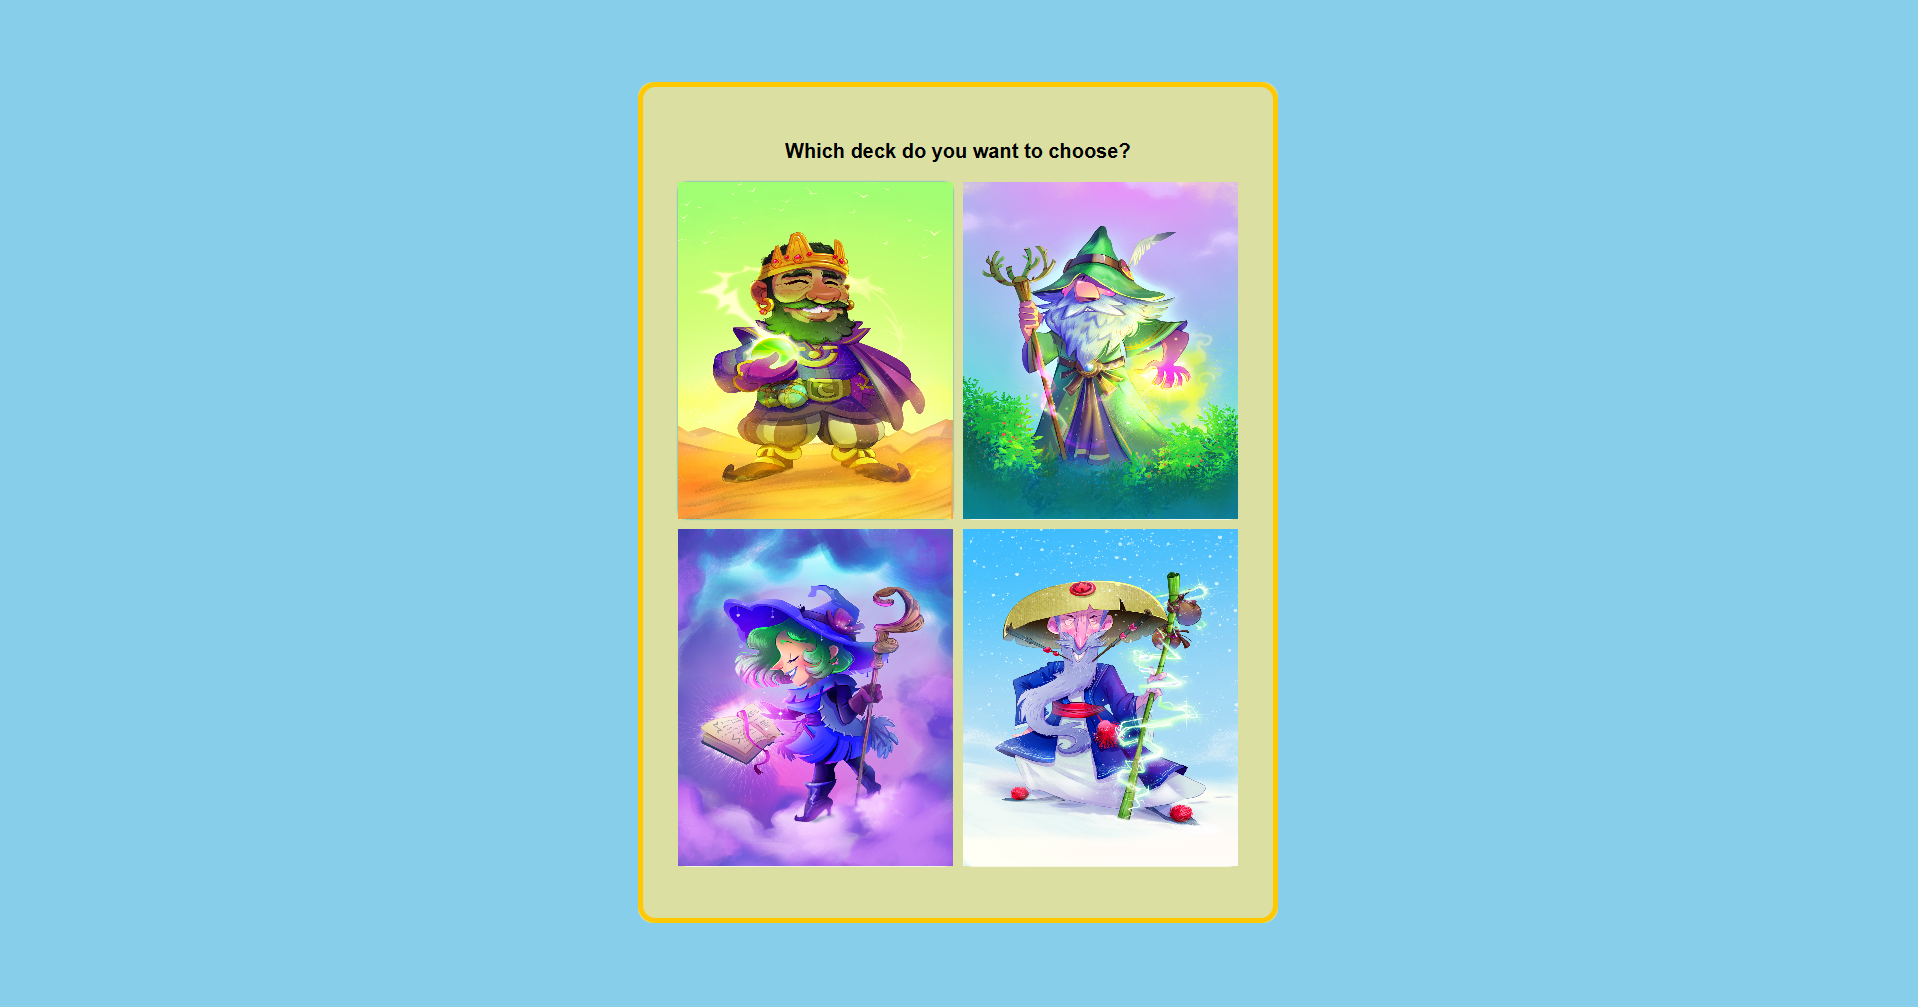
\includegraphics[width=\linewidth]{gui2Week9.png}
			\caption{GUI Scelta del Deck}
		\end{minipage}\hfill
		\begin{minipage}{0.495\textwidth}
			\centering
			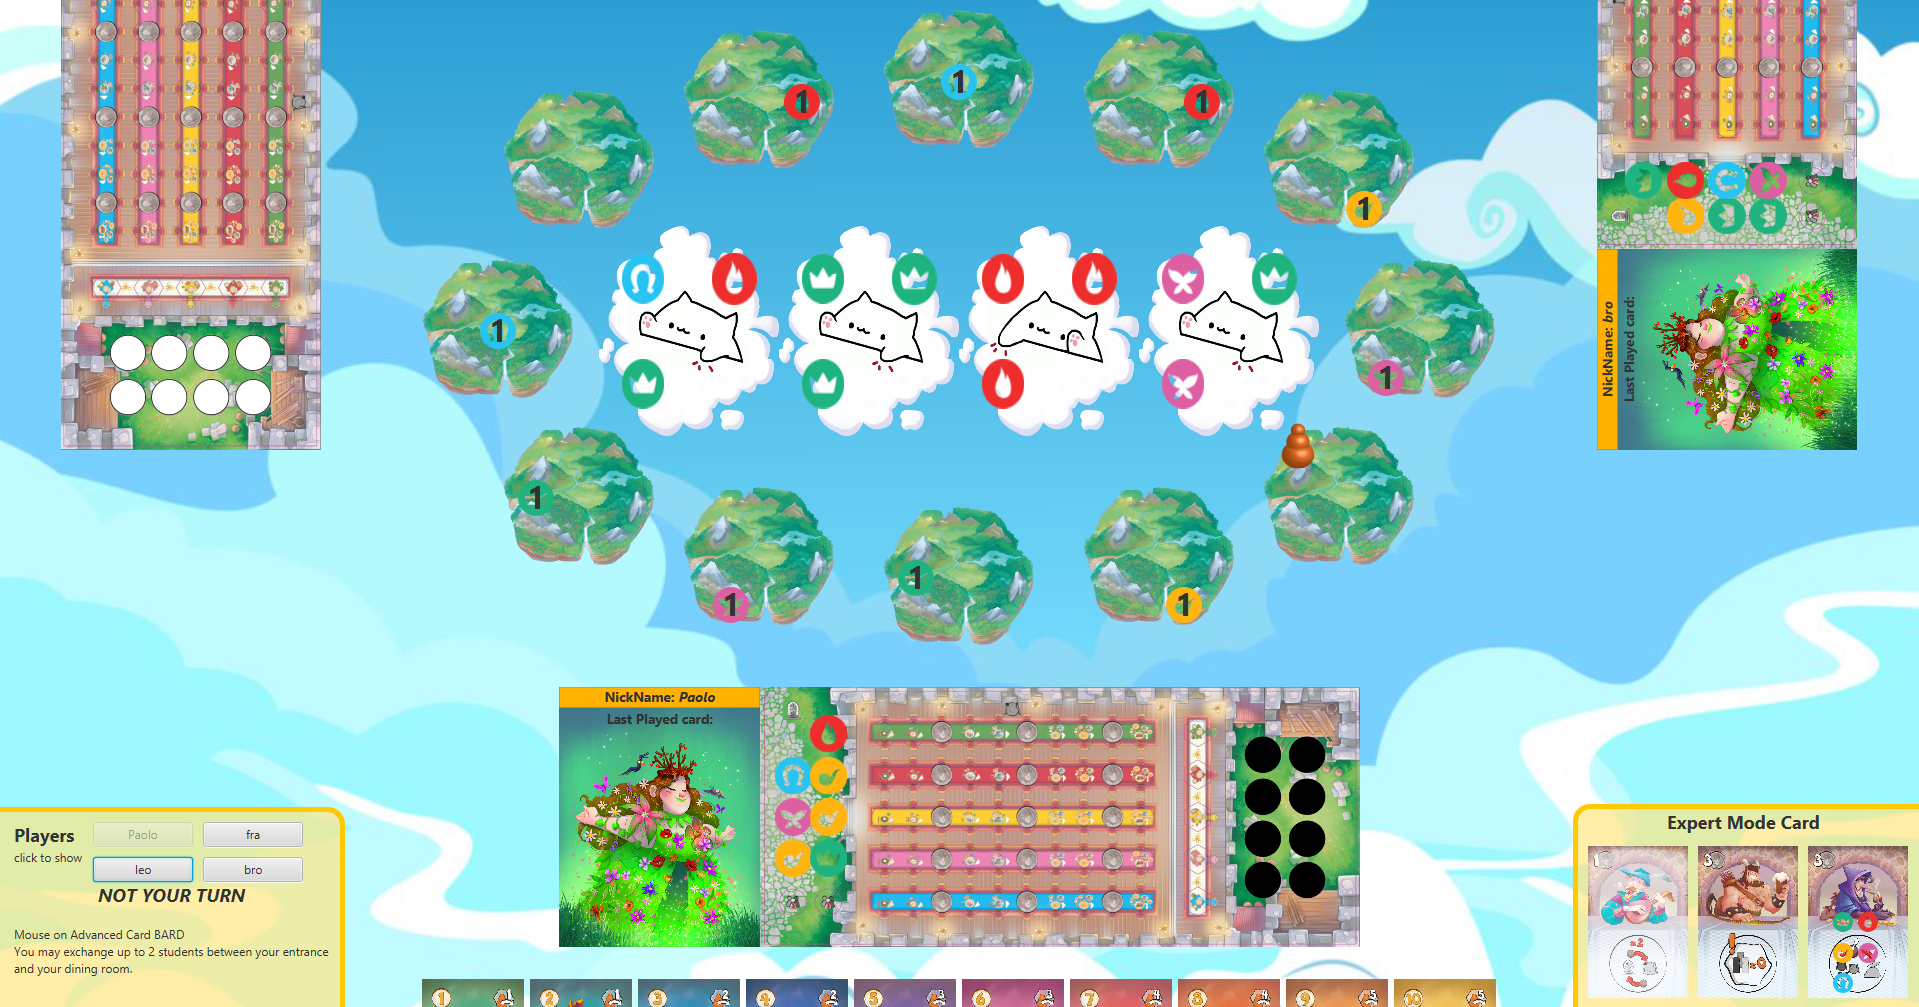
\includegraphics[width=\linewidth]{guiWeek9.png}
			\caption{GUI Board di gioco}
		\end{minipage}
	\end{figure}
	\paragraph{}
	La GUI è ancora in evoluzione. Nelle prossime settimane elaboreremo una nuova versione del client pre-partita.
	
	\newpage
	\subsection{Settimana 10: Launcher Update}
	\paragraph{}
	Nella decima settimana di sviluppo, è stato sviluppata una nuova versione del launcher, il quale gestisce tutte le interazioni con l'utente, dalla connessione al server, alla creazione o join di una lobby, alla scelta del proprio Mago con cui giocare. Di seguito qualche screen:
	\begin{figure}[!htb]
		\begin{minipage}{0.495\textwidth}
			\centering
			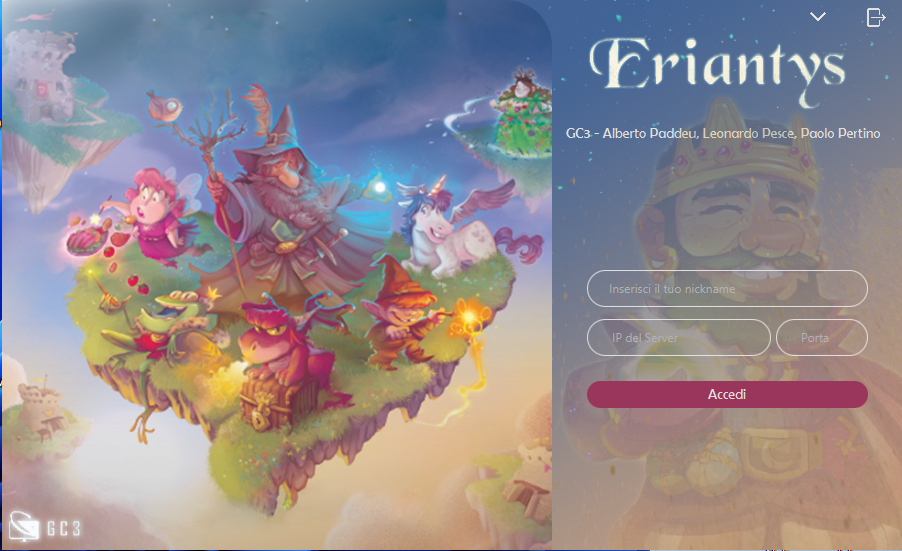
\includegraphics[width=\linewidth]{launcher_1.png}
			\caption{Pagina di login}
		\end{minipage}\hfill
		\begin{minipage}{0.495\textwidth}
			\centering
			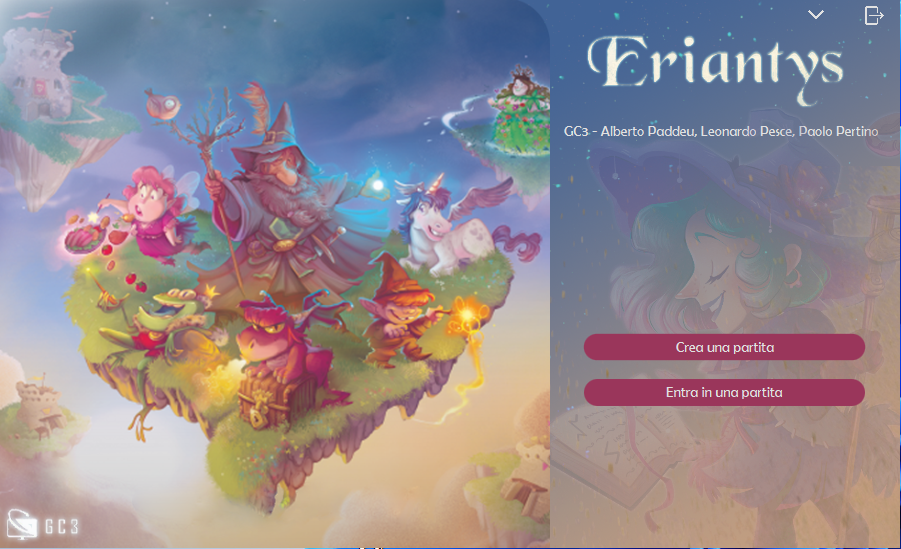
\includegraphics[width=\linewidth]{launcher_2.png}
			\caption{Launcher Menu}
		\end{minipage}
	\end{figure}
	\begin{figure}[!htb]
		\begin{minipage}{0.495\textwidth}
			\centering
			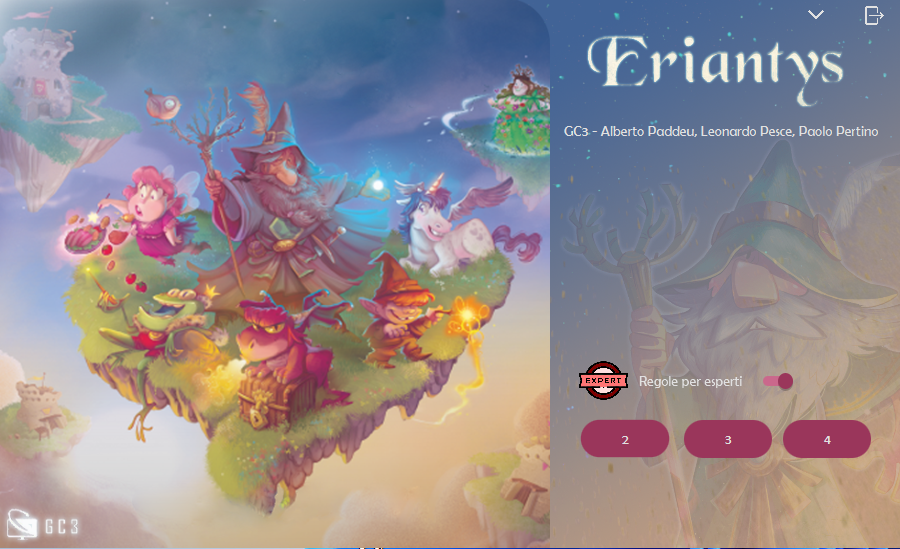
\includegraphics[width=\linewidth]{launcher_3.png}
			\caption{Creazione partita}
		\end{minipage}\hfill
		\begin{minipage}{0.495\textwidth}
			\centering
			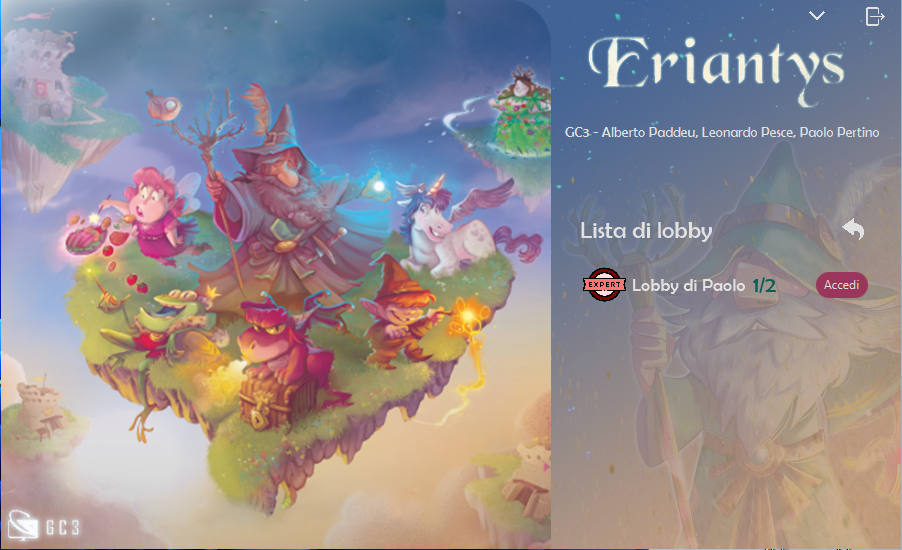
\includegraphics[width=\linewidth]{launcher_4.png}
			\caption{Accesso a partita}
		\end{minipage}
	\end{figure}
	\begin{figure}[!htb]
	\begin{minipage}{0.495\textwidth}
		\centering
		\includegraphics[width=\linewidth]{launcher_6.png}
		\caption{Scelta del mago}
	\end{minipage}\hfill
	\begin{minipage}{0.495\textwidth}
		\centering
		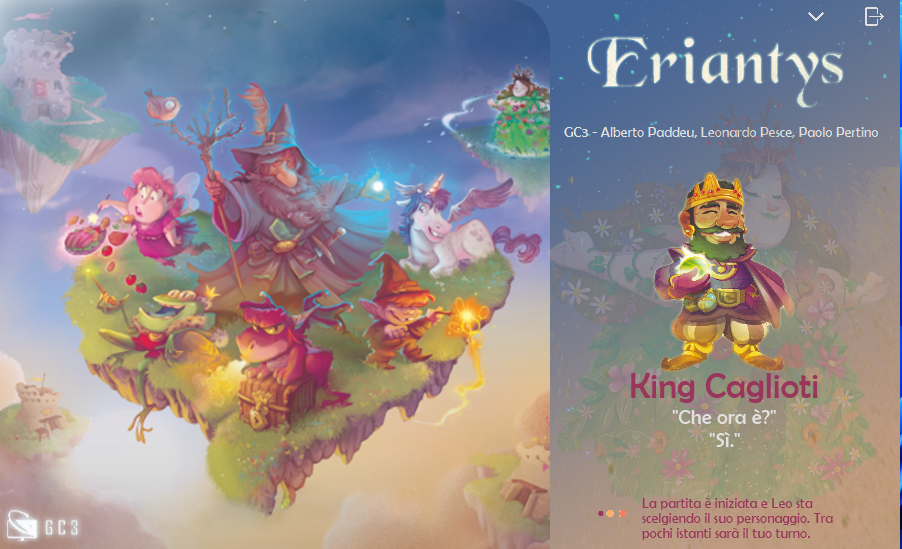
\includegraphics[width=\linewidth]{launcher_7.png}
		\caption{Mago scelto}
	\end{minipage}
	\end{figure}
	\paragraph{}
	Nelle prossime settimane creeremo appositi pop-up per messaggi come la disconnessione di uno dei giocatori dal server durante una partita, o la vittoria di un giocatore.
	
	\newpage
	\subsection{Settimana 11: Ulteriore testing e bugfixing}
	\paragraph{}
	Nel corso dell'undicesima settimana di sviluppo il team si è particolarmente concentrato sul testing delle partite a 4 giocatori e sulle winning condition secondarie (giocate tutte le carte assistente o pescati tutti gli studenti dalla bag).\\
	Inoltre sono stati risolti problemi legati alla visualizzazione dell'interfaccia da linea di comando e fixati altri bug sia lato client sia lato server.\\
	Abbiamo aggiunto una musica di sottofondo e aggiornato la fase di caricamento del gioco, inserendo un video che anticipa l'inizio della partita vera e propria (permettendo di caricare il file FXML della board in background e quindi evitando momenti morti di caricamento indesiderati).\\
	Infine il gioco è stato testato su 2 sistemi operativi differenti, ovvero \textit{Windows 11} e \textit{Ubuntu 22.04}.
	\paragraph{}
	Nel corso delle prossime settimane verrà ultimata la presentazione dei messaggi di errore nella GUI in appositi infobox e verrà gestita la terminazione della partita.
	
	\subsection{Settimana 12: Documentazione}
	\paragraph{}
	Nella dodicesima ed ultima settimana di sviluppo, il gruppo si è focalizzato sulla documentazione del codice e sull'aggiornamento dei diagrammi UML rimasti inalterati dalla settimana 8. Inoltre sono stati risolti alcuni bug grafici ed è stata gestita la terminazione della partita (vittoria, sconfitta, parità disconnessioni di altri client, disconnessione del server). Sono stati compilati i documenti README e le pagine relative alla Wiki sulla repository github per fornire istruzioni dettagliate su installazione e lancio del gioco.
	\paragraph{}
	Riteniamo dunque che il nostro materiale sia pronto per la consegna.
	
	% Strumenti usati
	\newpage
	\section{Strumenti utilizzati}
	Nella seguente sezione verranno indicati i principali strumenti di sviluppo utilizzati:\\
	\begin{itemize}
		\setlength{\parskip}{0pt}
		\setlength{\parsep}{0pt}
		
		\item \emph{IntelliJ IDEA Ultimate 2021.3.2} - Principale IDE utilizzato.
		\item \emph{Maven} - Gestione dello sviluppo del progetto software e di tutte le sue fasi.
		\item \emph{JUnit} - Framework principale di unit testing.
		\item \emph{SonarQube} - Analisi della qualità del codice.
		\item \emph{AstahUML} - Creazione di class diagram UML.
		\item \emph{sequencediagram.org} - Creazione di sequence diagram UML.
		\item \emph{GitKraken} - Git GUI per visualizzare il workflow di sviluppo ed utilizzare efficientemente Git.
		\item \emph{TEXStudio} - Gestione e aggiornamento del report.
	\end{itemize}

	% Bibliografia
	\newpage
	\begin{thebibliography}{99}
		\bibitem{eriantys}
		\href{https://www.craniocreations.it/prodotto/eriantys/}{Eriantys, Cranio Creations}
		
		\bibitem{carolusMagnus}
		\href{https://www.goblins.net/giochi/carolus-magnus-5071}{Carolvs Magnvs, Winning Moves} 
		
		\bibitem{circularDoublyLinkedList}
		\href{https://www.softwaretestinghelp.com/doubly-linked-list-in-java/#Circular_Doubly_Linked_List_In_Java}{Circular Doubly Linked List}
		
		\bibitem{javaUtilTimer}
		\href{https://docs.oracle.com/javase/7/docs/api/java/util/Timer.html}{Timer} - Documentazione Timer Java Util
		
	\end{thebibliography} 
\end{document}         
